\section{引言}\label{ux5f15ux8a00}

可扩展光子计算标志着高性能系统架构的一次关键转变,这一转变由人工智能日益增长的能源需求和电子互连的物理极限所驱动。随着数据密集型工作负载日益主导计算格局,传统依赖电荷传输的方式在带宽密度和能效方面面临着根本性的瓶颈。集成光子学提供了一种极具吸引力的替代方案,它利用光的固有并行性执行线性代数运算,从而可能将每次操作的能耗降低数个数量级。然而,从孤立的器件演示向晶圆级可编程系统的过渡不仅仅是增加组件数量的问题。它需要驾驭一个复杂的局面,其中包括材料权衡、架构约束以及定义当前 ODNN 研究现状的系统性物理限制。

材料平台的选择是可扩展光子系统的基石,对性能施加了根本性约束。硅光子学凭借其与互补金属氧化物半导体(CMOS)制造生态系统的兼容性,仍是高密度集成的首选方案,但其电光效应较弱,且在高功率下存在非线性损耗。相反,薄膜铌酸锂(TFLN)展现出更优的调制效率和低损耗特性,近期在下沉式双层电极设计方面的进展表明,其半波电压-长度乘积已低于 1.6 V \(\cdot\) cm \citep{doi_10_3390_photonics12111129_03f4b6cd}。然而,TFLN 目前尚缺乏用于大规模逻辑集成所需的成熟代工基础设施。这种二元对立表明,目前没有任何单一材料平台能同时满足规模、速度和能效的所有要求,因此需要采用混合集成策略,将不同材料整合在同一衬底上。

基于这些物理基础,可编程光子电路架构已成为实现可重构线性变换的主要机制。马赫-曾德尔干涉仪(MZI)网格作为典型的构建模块,能够实现通用酉变换,这对于光子神经网络和量子信息处理至关重要。在通用硅光子平台上的最新实验演示验证了对六边形波导网格的编程能力,对于小规模酉矩阵实现了超过 98\% 的保真度 \citep{doi_10_1063_5_0235712_fb28986d}。这些架构使得构建光子矩阵乘法引擎成为可能,该类引擎利用光学干涉执行并行点积运算。尽管此类引擎在低精度推理中展现出每 MAC(乘加运算)能耗方面的变革性优势,但由于被动介质中缺乏原生非线性,其适用性受到结构限制。因此,光子加速器最适合作为静态或缓慢变化的线性变换的专用协处理器,而非电子图形处理器的通用替代品。

尽管具备这些令人鼓舞的能力,实际光子计算系统的可扩展性受到累积物理效应的制约,这些效应会降低密集阵列中的信号保真度。光学深度神经网络(ODNN)研究中的主要张力源于光学计算的理论效率与热串扰、级联插入损耗以及制造诱导变异等现实挑战之间的冲突。在密集的可编程网格中,热光相移器会引入显著的热串扰,扰动相邻单元,从而需要复杂的校准协议,这削弱了节能优势 \citep{doi_10_1109_access_2020_3013116_8fec1fb2}。此外,缺乏高效的全光激活函数迫使人们依赖混合光电接口进行非线性操作,由此引入的延迟和功耗开销可能会抵消理论增益。对于需要频繁权重更新和梯度计算的动态训练负载而言,这一问题尤为严峻,因为光学硬件的刚性与其算法需求之间存在根本性的不匹配。最近对光子 Transformer 加速器的分析突出了这些挑战,指出虽然卷积工作负载能很好地映射到静态光子核心,但基于注意力的机制需要动态重配置,而当前硬件难以高效支持这一需求 \citep{doi_10_1109_hpca57654_2024_00059_f488ee7a}。

本综述综合了电子 - 光子协同设计这一新兴范式,该范式将硬件几何结构、控制电子学与算法架构视为一个统一的优化问题,以解决这些系统性瓶颈。协同设计方法并非孤立地优化器件,而是利用物理信息机器学习和逆向设计工具,自动将抽象的计算目标映射为可制造的器件几何结构。智能设计自动化框架(例如将制造感知逆向设计与布线感知布局相结合的框架)正开始弥合理论性能与实际可实现性之间的差距 \citep{doi_10_1117_12_3066105_d6297c38}。由此产生的设计延伸至系统级应用,其中光互连网络为带宽瓶颈提供了可立即部署的解决方案。OptoLink 等架构展示了光子互连在缓解专用加速器内存带宽约束方面的潜力,与电网络相比,其在显著降低延迟的同时实现了太比特级的吞吐量 \citep{doi_10_1145_3806395_315ab915}。

本综述遵循从物理约束到系统级解决方案的逻辑递进。S01节确立了支配器件性能的材料物理机制,随后S02节和S03节分别详细阐述了可编程架构和矩阵乘法引擎。S06节批判性地审视了由损耗、串扰和控制复杂性所定义的问题空间中的可扩展性瓶颈。随后,S07节提出了电子-光子协同设计方法作为应对这些挑战的战略响应。最后,S04节和S05节评估了AI加速和光互连中的系统级应用,并在S08节总结了ODNN研究的发展轨迹,指出了基准测试和标准化方面的关键空白。通过这种结构化分析,我们认为,可扩展光子计算的未来不在于器件指标上的孤立突破,而在于异构平台、智能设计算法和严格系统级验证的协同集成。

\section{用于可扩展光子计算集成的器件物理与材料平台}\label{ux7528ux4e8eux53efux6269ux5c55ux5149ux5b50ux8ba1ux7b97ux96c6ux6210ux7684ux5668ux4ef6ux7269ux7406ux4e0eux6750ux6599ux5e73ux53f0}

可扩展的光子计算设计空间从根本上由硅光子学与薄膜铌酸锂(TFLN)之间的材料二分法所塑造。硅光子学提供了一种高密度、CMOS 兼容的平台,对于密集集成至关重要,但其本质上受限于缺乏线性电光效应以及在高原光强下显著的双光子吸收损耗。\citep{doi_10_3390_photonics11040375_bd102ef0} \citep{doi_10_3390_photonics12010005_5e399e5f} 相比之下,TFLN 利用了铁电晶体特有的强普克尔斯电光调制和低传播损耗,使其适用于高速、能效高的操作,尽管目前在实现与硅相当的集成密度方面仍面临挑战。\citep{doi_10_3390_photonics12111129_03f4b6cd} \citep{doi_10_3390_mi17060751_d3932b5d} 介于这两者之间,氮化硅在 1.55 \(\mu\) m 处表现出约为 2.5 \(\times\) 10\(^{-19}\) m\(^{2}\)/W 的非线性 susceptibility,能够实现高效的四波混频过程,适用于克尔微梳产生等应用。此外,氮化硅在可见光和近红外光谱窗口具有超低传播损耗,尽管其微弱的电光响应同样需要辅助调制方案。这种权衡造成了一个关键瓶颈:虽然硅受益于成熟的制造生态系统,但其对热光相移器的依赖引入了不可避免的热串扰,可能导致信号路由错误,并限制了其在密集网络中的工作能力。因此,材料平台的选择制约了集成电路可实现的规模、速度和能效,迫使采用混合集成策略以平衡制造成熟度、损耗和速度之间的相互冲突的需求。\citep{doi_10_48550_arxiv_2209_10098_b3bedb78} \citep{doi_10_1126_science_abj4396_40f36a09} \citep{doi_10_1149_ma2026_01311465mtgabs_643e381a} \citep{doi_10_1109_access_2020_3013116_8fec1fb2}

矩阵向量乘法(MVM)作为光神经网络的核心运算,其实现依赖于由既往材料限制所确立的三种主流架构基元:自由空间衍射系统、马赫 - 曾德尔干涉仪(MZI)阵列以及微环谐振器(MRR)网络。\citep{doi_10_1088_1402_4896_ae8345_3b948559} 自由空间系统利用衍射层执行计算,虽具备高吞吐量,但本质上体积庞大,难以片上集成,且针对可扩展应用的调谐极具挑战。相比之下,基于 MZI 阵列和 MRR 的集成方案提供了适用于芯片级光子计算的紧凑结构,却引入了独特的物理脆弱性。这些集成方法需要极高精度的相位控制和复杂的反馈电路才能运行,往往面临功耗高、稳定性差的问题,并受到波导串扰和传输损耗所施加的可扩展性限制。第三条路径,即衍射光神经网络(DONNs),应运而生以弥合上述差距;DONNs 最初开发于自由空间,如今已转向片上实现以增强与光子电路的兼容性,提供无源低功耗运行和超高吞吐量。然而,与其集成对应方案类似,这些片上衍射架构必须克服复杂的光学约束以实现可重构性。归根结底,在这些架构之间的选择代表了集成器件的可扩展性与可编程性同自由空间系统的庞大体积及调谐困难之间的关键权衡,这也为限制其大规模部署的热稳定性和制造稳定性挑战埋下了伏笔。\citep{doi_10_1088_1402_4896_ae8345_3b948559} \citep{doi_10_1002_nap2_70098_8d5f2f8a}

图 \ref{fig:visual_01}展示了本节讨论的代表性视觉证据。

\begin{figure}
\centering

\includegraphics[width=0.9\linewidth,height=\textheight,keepaspectratio,alt={Photonic Material Platform Trade-off Landscape. No single platform dominates all metrics, requiring selection based on specific computing workload priorities like speed versus integration density. AI-assisted explanatory diagram; not empirical evidence.}]{figures/01_FIG-GEN-001.png}
\caption{Photonic Material Platform Trade-off Landscape. No single platform dominates all metrics, requiring selection based on specific computing workload priorities like speed versus integration density. AI-assisted explanatory diagram; not empirical evidence.}\label{fig:visual_01}
\end{figure}

材料平台固有的物理噪声源在扩展复杂矩阵运算时,会从根本上降低马赫-曾德尔干涉仪(MZI)阵列等架构基元的保真度。在硅光子集成电路中,热串扰源于芯片材料不可避免的热导率,即对某一组件的加热会在相邻波导中产生不需要的相移。\citep{doi_10_1109_access_2020_3013116_8fec1fb2} 这种现象是热光相移器和衰减器密集阵列中的主要误差机制,可能导致信号路由错误和输出功率降低。尽管已提出三维沟槽或掺杂硅加热器等策略以局部化加热效应,但通过硅衬底的热耗散限制了全面的分析。除了这些热学问题外,制造偏差------特别是波导宽度和厚度的有限精度------引入了破坏相干纳米光子神经网络中矩阵向量乘积的基本相位噪声。\citep{doi_10_1109_tnano_2022_3223915_d4da3e6b} 这些器件对这类偏差的灵敏度与标称尺寸成正比,尽管优化的脊形波导设计显示出对预期不均匀性的抵抗力。此外,虽然光子谐振器为实现激活函数提供了有利的非线性行为,但它们极易受到温度波动和机械振动等环境因素的影响,因此需要复杂的控制机制来维持稳定性。热管理、制造公差和环境敏感性这些相互交织的限制表明,光子计算的扩展既是一个设计挑战,也是一场对抗固有物理局限的斗争。\citep{doi_10_1109_access_2020_3013116_8fec1fb2} \citep{doi_10_1109_tnano_2022_3223915_d4da3e6b} \citep{doi_10_3390_nano14080697_c372a140}

异质后道工艺(BEOL)集成已成为一种核心的统一策略,旨在解决此前在尺寸缩放壁垒中所识别出的高速调制与高密度 CMOS 兼容布线之间的相互冲突需求。该方法涉及在标准硅电路制造完成后,将具有强普克尔斯电光效应的薄膜铌酸锂(TFLN)直接键合到有源硅光子平台上。\citep{s2_9b444e84d20ae6e3d62d2d4df30268b5a53baad2_40af2cc9} 通过结合这些层级,该平台既利用了 TFLN 固有的低损耗和卓越的调制效率,又保留了硅光子学成熟且高度集成的设计套件,以实现高密度布线和探测。近期的演示证实,该光学架构克服了关键的芯片到晶圆(die-to-wafer)键合挑战,成功将高性能调制器与锗光电探测器集成在同一芯片上,为面向片上光网络的可扩展收发器开辟了清晰路径。作为这种垂直堆叠的补充,片上介电超表面提供了一种独特的方案,能够在紧凑的占位面积内调控光场的自由度。这些超表面与标准 CMOS 工艺兼容,可作为任意波前整形器执行卷积等模拟数学运算,从而成为宽带、低损耗光子计算加速器的有力候选者。为了展示这一能力,研究人员基于非对称光子自旋 - 轨道相互作用开发了一种单片超表面空间微分器,用于执行边缘检测。该器件利用偏振自由度工作,并在宽带范围内运行,为庞大的光学模拟系统提供了一种更紧凑的替代方案。\citep{doi_10_1515_nanoph_2020_0366_58f1aa1d} 尽管超表面器件的可重构性仍是当前活跃的研究领域,但异质 BEOL 集成与超表面功能的融合阐明了一个克服材料二元对立的关键方向:即合并不同平台的最佳物理属性以实现晶圆级系统,尽管这些混合策略的全面实现仍需进一步的方法论发展。\citep{s2_9b444e84d20ae6e3d62d2d4df30268b5a53baad2_40af2cc9} \citep{doi_10_1515_nanoph_2022_0294_1bd118d5}

逆向设计方法论通过直接从所需光学响应确定最优几何结构,解决了传统器件布局中固有的几何刚性问题,从而补充了旨在解决材料冲突的混合集成策略。\citep{doi_10_1364_oe_524318_cf5f0d79} \citep{doi_10_1364_ol_453299_4bc70b17} 与传统的直觉驱动设计不同,该方法采用优化算法和深度学习来探索复杂的参数空间,生成满足特定性能目标的结构,并通过创建对微小几何变化不敏感的鲁棒模式来缓解制造公差限制。其机制通常依赖于用深度学习代理模型取代计算密集型电磁仿真(如蒙特卡洛或时域有限差分求解器),从而实现对闪烁体和功率分配器等复杂几何结构的高效梯度优化。\citep{doi_10_1109_jmmct_2026_3695747_9d633c4d} \citep{doi_10_17725_j_rensit_2026_18_163_741010b8} 然而,这种灵活性并非绝对;可访问的设计空间仍严格受限于制造公差,特别是最小特征尺寸和长度尺度限制。例如,使用粗网格来强制执行这些约束的方法会将搜索范围局限于极少量的可能结果,导致所得最优结构的效率显著低于在更广泛、物理信息驱动的设计空间中发现的结构。此外,尽管人工智能在经过训练后能快速生成优化设计,但该过程需要大量的初始仿真数据,产生了随结构复杂度增加的显著一次性计算成本。最终,这些人工智能生成器件的性能无法超越其训练数据集所蕴含的能力上限,这表明逆向设计是驾驭材料平台权衡的强大工具,但需仔细管理计算资源和物理边界,以实现可扩展的光子计算。\citep{doi_10_1515_nanoph_2024_0536_4b6631ba} \citep{doi_10_1515_nanoph_2023_0852_cb27a26f} \citep{doi_10_1109_cleo_europe_eqec65582_2025_11110329_26a41a7d}

逆向设计算法能有效导航复杂的几何空间,但其对传统数值求解器的依赖为晶圆级电路带来了计算瓶颈。深度学习代理模型通过用快速的神经网络近似取代昂贵的频域有限差分仿真来解决这一问题。具体而言,神经算子作为一种强大的框架应运而生,它学习函数空间之间的映射关系,例如将材料系数或边界条件作为输入,直接返回解场,而非回归固定维度的向量。\citep{doi_10_48550_arxiv_2303_10506_0452bde4} 一旦训练完成,这些模型能以可忽略的成本评估新设计,同时保持可微性,这一特性对于基于梯度的优化至关重要。实际实现展示了这一效率;例如,在数千个仿真数据点上训练的深度神经网络可以在不到一秒的时间内预测集成光子功率分配器的光谱响应,从而实现快速逆向设计,即用户指定的光学响应能立即映射到器件拓扑结构。代理散射矩阵逆向设计通过利用学习到的模型绕过传统仿真瓶颈,实现了光子神经网络的可扩展构建。\citep{s2_753a5d83a96e0194da93bcb6f20fa0bd356e37fa_c11e3796} 此外,物理信息方法和伴随方法利用这些能力来处理偏微分方程约束的最优控制问题,为克服传统仿真工作流中固有的扩展极限提供了途径。通过将设计迭代与繁重的数值求解解耦,这些代理模型提供了实现可扩展光子计算所需的密集、高性能架构所必需的计算速度。\citep{doi_10_48550_arxiv_2601_00199_c689b34d} \citep{doi_10_1038_s41598_018_37952_2_076b64f9} \citep{doi_10_48550_arxiv_2606_12337_68b62bfa}

神经代理模型在加速候选设计生成方面的效用从根本上受到泛化极限和光子目标景观崎岖拓扑的限制。深度学习框架往往难以外推至超出其训练数据集中特定几何结构和光谱的范围,限制了其在缺乏额外细化情况下提出新颖结构的能力。为了克服这一局限,混合算法应运而生,将用于全局搜索的神经网络与常规优化方法(如基于伴随的技术)相结合,以执行局部细化。此外,光子器件的物理性质引入了严峻的数学挑战;例如,在分布式布拉格反射镜中,波之间的循环干涉会产生高度振荡的目标函数,其中充斥着使 Adam 或 L-BFGS 等标准基于梯度的优化器陷入困境的局部极小值。尽管人工智能显著加快了设计周期,但这些输出的可靠性仍然取决于底层物理模型的保真度以及通过电磁仿真生成足够训练数据的计算成本。因此,实现稳健的晶圆级集成需要超越纯数据驱动的方法,转向能够导航这些不规则损失景观并在多种材料平台上泛化的方法。\citep{doi_10_1021_acsphotonics_2c00968_06a2e96b} \citep{doi_10_48550_arxiv_2602_18148_e9c0a72b} \citep{doi_10_1515_nanoph_2024_0536_4b6631ba}

光深度神经网络(ODNN)研究正趋向于融合混合集成与人工智能驱动的反向设计,以克服前文所述的材料与制造瓶颈。物理信息机器学习成为管理晶圆级光子电路复杂性的关键赋能技术,使得在高维设计空间和严格制造限制下仍能优化器件性能。通过将支配性物理定律直接嵌入学习过程,这些方法降低了对数据的依赖性;而混合框架则将深度学习与伴随法等经典优化技术协同结合,以确保稳健收敛。例如,成本效益高的深度学习代理模型已成功针对特定衍射目标优化了超原子几何结构, navigated 固定材料高度和光刻分辨率限制等约束,而这些约束往往会阻碍传统迭代方法。这种计算优势与光子集成电路(PICs)的物理优势相辅相成,后者相比传统电子系统提供了更卓越的能效和可扩展性,特别是在通过大规模并行处理解决旅行商问题等组合优化问题时。最终,实现可扩展光子计算的路径并非依赖单一突破,而是取决于这一双重策略:利用智能算法最大化异质材料平台的潜力,从而将物理约束转化为可管理的设计参数。\citep{doi_10_1109_sbfotoniopc62248_2024_10813471_692f0088} \citep{doi_10_1021_acsami_5c03196_32a62b73} \citep{doi_10_3390_nano14080697_c372a140}

\section{用于光子计算的可编程光子电路架构与可重构网格拓扑}\label{ux7528ux4e8eux5149ux5b50ux8ba1ux7b97ux7684ux53efux7f16ux7a0bux5149ux5b50ux7535ux8defux67b6ux6784ux4e0eux53efux91cdux6784ux7f51ux683cux62d3ux6251}

可编程光子计算以马赫-曾德尔干涉仪(MZI)网格为基本构建模块,通过精确的相位控制干涉实现通用酉变换。\citep{doi_10_48550_arxiv_2407_03235_fe345c4b} \citep{doi_10_1063_5_0235712_fb28986d} 在这些相干阵列中,光束被分束、经历可调相位偏移并重新组合,从而以光速直接执行线性代数运算。该架构已成为集成芯片上光学矩阵向量乘法的主流解决方案,与自由空间衍射系统和微环谐振器网络并列,作为在后摩尔时代突破电子加速器带宽和能效限制的主要途径。借助硅光子学技术,基于MZI的系统有望显著降低矩阵运算的复杂度,并为推理任务提供近乎零延迟的性能。然而,尽管作为传统电子学的潜在替代方案前景广阔,这些集成解决方案在向高密度集成扩展时面临重大瓶颈:它们需要极其精确的相位控制和复杂的反馈电路,且易受制造工艺变化的影响,若无单独校准,可能导致灾难性的精度损失。理论上的通用变换能力与实际稳定性及控制挑战之间的张力,定义了当前可编程光子架构的研究格局。\citep{doi_10_1109_tnano_2022_3223915_d4da3e6b} \citep{doi_10_1088_1402_4896_ae8345_3b948559}

衍射光学神经网络(DONNs)提供了一种静态、无源的替代方案,以取代可编程的马赫-曾德尔干涉仪网格,后者通过主动调谐实现通用酉变换。DONNs通过物理衍射层实现线性变换,与可重构但功耗较高的干涉阵列不同,它利用其在神经元数量和超高吞吐量方面的可扩展性,为特定机器学习任务实现低功耗运行,其发展已从基础的自由空间实现演进为与光子电路兼容的片上集成配置。该领域的一个代表性进展是光子晶体衍射光学神经网络(PhC-DONN),它利用二维光子晶体实现多波长并行处理,用于片上光学分类。通过建立波长-衍射联合调制模型,PhC-DONN克服了传统单波长衍射网络的固有局限性,在图像和视频分类方面表现出卓越性能,并为高效光学人工智能处理器提供了一条路径。虽然这些静态架构缺乏MZI网格的动态可重构性,但其以极低能耗执行固定线性操作的能力凸显了光子计算设计中的一个关键权衡,也为超越人类直觉进一步优化此类非标准拓扑结构的逆向设计技术奠定了基础。\citep{doi_10_1002_nap2_70098_8d5f2f8a} \citep{doi_10_1515_nanoph_2025_0168_86a0f7aa}

超越静态衍射网络的固定变换和标准马赫-曾德尔干涉仪(MZI)阵列的规则几何结构,纳米光子学逆向设计代表了一种范式转变,克服了基于直觉的手工工程固有的局限性。\citep{doi_10_1088_1361_6633_ae7f9a_e05f9b1d} \citep{doi_10_1109_icufn61752_2024_10625552_985a60f2} 这种计算方法直接从所需的光学响应确定器件几何形状,从而能够实施传统启发式方法无法构想的非直观电路拓扑。与依赖重复模拟循环进行渐进式改进的传统试错建模不同,逆向设计算法遍历整个参数空间以最小化成本函数,经常揭示出具有最佳性能且违背人类几何预期的复杂结构。人工智能和深度学习的集成进一步加速了这一过程;虽然生成初始训练数据集需要大量的计算努力,但经过训练的神经网络随后可以几乎即时地解决设计请求。这些数据驱动模型捕捉了材料属性与光学响应之间复杂的物理关系,允许同时优化更高层级的性能优值并快速收敛设计参数。通过将优化方案与深度学习预测器融合,研究人员现在可以有效地在复杂的能量景观中探索全局最优解,从根本上改变了为最大化计算密度和功能而构思可编程光子架构的方式。\citep{doi_10_1515_nanoph_2021_0660_2d91a441} \citep{doi_10_1515_nanoph_2018_0183_d85e9193}

深度神经网络现已成为关键的代理模型,加速了集成纳米光子器件的发现,这一进展建立在从直觉驱动布局向算法逆向设计转变的基础之上。该实现的核心在于利用训练好的网络取代计算繁重的数值模拟,这些网络既能将器件几何参数直接映射为光学响应,也能反向预测针对特定光谱输出最优的纳米结构。例如,ResNet 架构在经过数千个模拟数据点的训练后,已展现出在巨大设计空间内近似任意孔矢量光谱响应的能力,从而能够在几分之一秒内设计出优化的功率分束器拓扑。判别式模型专门规避了重复电磁输入 - 输出模拟的瓶颈,而生成式方法则通过学习一对多映射来解决欠约束问题,从而产生多样化的结构候选方案。这种多样性对于实际应用至关重要,它使研究人员能够选择形状更平滑、纵横比更低的设计,以符合纳米加工约束并表现出对工艺变化的鲁棒性。然而,这些数据驱动的工作流程并非没有局限;混合流水线往往仍是必要的,以便将昂贵的全波评估保留用于最终验证,确保快速生成的提案不违反物理约束或不受代理模型不准确性的影响。通过大幅降低探索非标准拓扑的计算成本,这些深度学习代理直接促成了可编程光子计算所必需的高密度、复杂电路架构,尽管它们的集成也带来了管理工作流程复杂性和确保物理一致性的新挑战。\citep{doi_10_1038_s41598_018_37952_2_076b64f9} \citep{doi_10_29026_oes_2022_210012_27973a69} \citep{doi_10_1109_access_2026_3697666_bd5258a6}

深度学习代理模型加速了评估过程,然而光子结构的底层逆向设计往往涉及具有振荡行为的复杂、不规则目标函数,这需要先进的优化策略以避免陷入局部极小值。例如,在分布式布拉格反射器中,反射波与透射波之间的干涉随层厚呈周期性变化,形成了一种优化景观,使得标准的梯度下降法或拟牛顿法(如 L-BFGS)若未经过谨慎初始化便难以收敛。\citep{doi_10_1515_nanoph_2020_0379_1cc596ab} 为应对这些挑战,研究人员采用了粒子群优化或协方差矩阵自适应进化策略等全局方法,尽管这些无梯度方法在高维应用中通常收敛较慢。新兴的混合贝叶斯优化框架结合了神经嵌入或学习到的潜在表示,以解决计算开销和超参数敏感性问题,从而 bridging 符号建模与深度表示学习。此外,包括物理信息神经网络(PINNs)在内的物理信息机器学习方法正被应用于求解与光子器件仿真相关的前向和逆向问题,通过将控制方程直接嵌入训练过程,可能降低网格校准的计算成本。然而,当前的生成式框架仍面临''约束严谨性差距'',在通过软惩罚施加硬物理约束时,其可行性比率往往低至 60-80\%,这表明纯数据驱动的映射必须进一步与数学约束严谨性相结合,才能完全取代迭代采样范式。\citep{doi_10_48550_arxiv_2602_18148_e9c0a72b} \citep{doi_10_48550_arxiv_2511_00070_bf8eda11} \citep{doi_10_48550_arxiv_2606_12337_68b62bfa}

先进的优化技术能够导航复杂的损失景观;然而,逆向设计光子电路的实际效用最终取决于其可制造性。为确保生成的拓扑结构符合标准晶圆厂工艺,必须在设计阶段明确施加制造约束(如最小特征尺寸)。这一要求将连续优化问题转化为组合挑战,可通过采用条件生成器和直通估计器来近似求解,从而在随机梯度下降过程中始终保持严格的长度尺度可行性。\citep{doi_10_1021_acsphotonics_2c00313_0d7d39c3} 相反,依赖启发式方法进行传输矩阵建模往往弊大于利;这些设计通常过度简化空间解耦的物理过程,导致产生无法实现的响应和显著的性能下降。尽管严格的''仿真在环''训练为实现物理可实现性提供了一条路径,但由于求解大型超表面麦克斯韦方程的计算成本高昂,该方法往往因费用过高而难以实施。因此,成功的架构设计需要在严格的几何约束与计算上可行的物理强制之间取得平衡,确保非直观拓扑的理论优势能够在物理硬件中得以实现。\citep{doi_10_1021_acsphotonics_2c00313_0d7d39c3} \citep{doi_10_48550_arxiv_2505_18377_a6fc9ec3}

这些经过优化的组件最终汇聚成集成光子张量核心,利用并行卷积处理架构来实现可编程计算基础的线性代数运算。与标准网格阵列不同,逆向设计的光子神经网络加速器采用紧凑的非网格拓扑结构,其中输入特征被编码到单一波长的相干光振幅上。逆向设计的光子神经网络加速器已被开发出来,旨在通过利用非网格拓扑结构实现超紧凑的光学计算。\citep{doi_10_1038_s41467_026_68648_1_26658a9c} 在拓扑优化的散射区域内,这些编码场经历复杂的干涉和散射相互作用,实现了光学能量的非均匀且空间自适应的传输,从而高效地将功率从输入编码端口直接路由至类别输出端口。该策略同样将器件体积视为衍射处理器,通过对每个端口处的光功率密度进行面积分归一化来计算输出概率分布,从而有效最小化交叉熵损失以限制通道串扰。通过在设计阶段对硅和二氧化硅强制执行二值化材料约束,这些加速器实现了无需后处理离散化的可制造几何结构,验证了本章的核心论点:非直观拓扑结构能够克服规则阵列的缩放限制,提供高密度计算单元。\citep{doi_10_1515_nanoph_2022_0423_38a2c3ec} \citep{doi_10_1038_s41467_026_68648_1_26658a9c}

扩展基于逆向设计的紧凑型张量核可编程网格遭遇了一个根本性的物理障碍:热串扰。\citep{doi_10_1109_access_2020_3013116_8fec1fb2} 这一现象源于芯片材料不可避免的热导率,即在密集光子电路中加热一个元件会导致其与相邻调谐组件产生非预期的耦合。在集成衰减器和交换网络中,此类热扩散可能导致光场限制失效、输出功率降低以及信号路由错误,从而实质上限制了器件的工作能力。尽管已提出多种缓解策略,但它们往往引入新的权衡;例如,超低损耗设计可能受限于较大的占地面积和高功耗,而时分复用寻址方案则受到最大可实现相移和电气设计参数的限制。即便是三维沟槽或专用热本征模分解等先进技术,也面临着定制化困难、需要外部散热器而阻碍标准 CMOS 工艺可行性、或通过硅衬底的热耗散分析不完整等挑战。因此,热串扰仍然是限制高密度可编程架构控制保真度和可扩展性的关键瓶颈,亟需在简单的几何紧凑化之外寻求进一步的创新。\citep{doi_10_1109_access_2020_3013116_8fec1fb2}

\section{光子矩阵乘法引擎作为可扩展光子计算中的核心计算单元}\label{ux5149ux5b50ux77e9ux9635ux4e58ux6cd5ux5f15ux64ceux4f5cux4e3aux53efux6269ux5c55ux5149ux5b50ux8ba1ux7b97ux4e2dux7684ux6838ux5fc3ux8ba1ux7b97ux5355ux5143}

光子矩阵乘法引擎被定义为核心计算单元,它通过光干涉执行线性变换,使得输出场振幅或强度与输入向量元素和可编程权重矩阵系数的点积成正比。\citep{doi_10_1109_hpca57654_2024_00059_f488ee7a} 与依赖电荷在电阻互连中移动的电子处理器不同,这些引擎利用光波的自然叠加,以光速执行并行乘加运算,其能耗主要由透射光功率而非电容充电决定。\citep{doi_10_1109_icop56156_2022_9911729_8d67554d} \citep{doi_10_1145_3716368_3735243_93c8da73} 这种物理机制实现了高吞吐量推理任务,正如集成光子张量核所证明的那样,它们利用级联可重构超表面或相干纳米光子电路来动态编码权重和输入,以实现片上处理。虽然静态衍射深度神经网络已成功在自由空间中实现全光机器学习,但现代方法优先考虑动态可重构、硅集成的器件,以克服适应性和集成密度方面的局限性。因此,光子引擎在低精度线性代数的能效方面具有理论优势,确立了其作为专用加速器的地位,而其潜力的充分发挥取决于克服组件微型化和无缝电子接口方面的障碍。\citep{doi_10_1088_1402_4896_ae8345_3b948559} \citep{doi_10_1515_nanoph_2022_0423_38a2c3ec} \citep{doi_10_3390_nano14080697_c372a140}

尽管光子线性代数在理论上具有能效优势,但其实际实现依赖于三种主要硬件拓扑结构:自由空间衍射系统、集成马赫-曾德尔干涉仪(MZI)阵列和微环谐振器(MRR)网络。自由空间方法利用衍射层执行并行操作,但由于其体积庞大且难以进行片上调谐,面临显著的集成挑战。相比之下,基于 MZI 阵列或 MRR 网络的集成解决方案提供了适合高密度封装的紧凑结构,但在可扩展性方面引入了不同的瓶颈。这些集成架构需要由复杂反馈电路支持的极精密相位控制,往往因波导串扰和光学损耗而导致功耗高、稳定性差以及性能下降。除了上述主要类别外,光子晶体通过采用周期性结构的介电复合材料来操纵电磁波传播,为纳米光子组件提供了另一种基础。\citep{doi_10_71465_gmssrj79_3a431fc8} \citep{doi_10_3390_axioms14060445_76ffad4a} 通过对光子能带结构进行工程化设计,这些周期性排列------从一维布拉格反射镜到二维平面阵列------可以禁止或允许特定频率范围的传播,从而实现对光色散的精确控制。\citep{doi_10_4302_plp_v17i4_1361_327bd6c2} \citep{doi_10_1149_ma2026_01231276mtgabs_21448056} 虽然钛酸钡等材料已成功用于制造此类结构,应用于太赫兹生成和滤波等领域,但架构的选择最终涉及物理尺寸与维持信号完整性复杂性之间的权衡,这为先进的逆向设计方法来优化这些相互制约的因素奠定了基础。\citep{doi_10_1088_1402_4896_ae8345_3b948559} \citep{doi_10_1002_adom_202001249_3b8c9743}

光子矩阵乘法引擎日益转向逆向设计,这是一种计算方法论:通过计算材料属性以产生特定的光学响应,而非优化预定义的形状,从而克服直觉设计的几何限制。\citep{doi_10_1364_oe_530479_45946046} \citep{doi_10_1117_12_2649964_b6e13b8f} 该设计利用拓扑优化和伴随方法等算法,高效计算损失函数相对于设计参数的梯度,从而发现传统启发式方法无法识别的复杂纳米光子结构。例如,逆向设计已成功应用于通过自由优化亚波长几何结构来制造超紧凑偏振分束器,从而扩展参数空间以实现满足严格晶圆厂制造约束并最小化器件占位面积的精细结构。通过物理约束逆向设计实现了超紧凑数字超表面偏振分束器,证明了针对紧凑器件占位面积优化亚波长几何结构的能力。\citep{doi_10_3390_app121910064_718c1a26} 此外,人工神经网络已成为该框架内的强大工具,用于优化集成纳米光子光学神经网络,在仅几平方微米的占位面积内实现均方误差低于10\^{}-4的高精度随机矩阵乘法。例如,一种基于光学散射单元的逆向设计光学神经网络,在紧凑的4 \(\times\) 4 \(\mu\) m\(^{2}\)占位面积内实现了均方误差低于10\^{}-4的高精度随机矩阵乘法。所提出的网络利用了这些单元在小区域内来回散射光的能力,与受摩尔定律限制的电子实现相比,具有速度快、功耗低的优点。\citep{doi_10_1016_j_scib_2020_03_042_6b632485} 虽然这些算法策略显著提高了组件密度和性能,但它们代表了向计算密集型设计阶段的转变,这是实现可扩展光子计算核心所需的紧凑、节能线性代数单元的必要条件。\citep{doi_10_1515_nanoph_2020_0379_1cc596ab} \citep{doi_10_3390_app121910064_718c1a26} \citep{doi_10_1016_j_scib_2020_03_042_6b632485}

生成式人工智能与物理信息神经算子如今在逆设计算法基础之上,大幅降低了复杂光子结构工程的计算成本。例如,自回归模型通过对设计参数间的条件依赖关系进行建模,顺序生成超材料几何结构,即基于已生成的令牌有效预测每个结构单元,以满足相位控制或光谱保真度等特定电磁目标。\citep{doi_10_48550_arxiv_2507_06853_b7161f49} 这种顺序合成方法已扩展至基础模型架构,该架构统一了表示学习与条件生成,能够为单一目标响应产生多种可行的结构。作为对这些生成方法的补充,受物理启发的神经算子通过提供电磁动力学的超快近似,解决了传统有限元仿真运行时间过长的问题。\citep{doi_10_1016_j_compositesb_2025_112935_31ebab19} PIC2O-Sim 等方法利用专用阶段模型和跨阶段隐藏状态传播,减轻了时间预测中的累积展开误差,从而在保持效率的同时确保了精度。\citep{doi_10_48550_arxiv_2406_17810_813bd2a3} 此外,物理感知神经网络可作为代理模型,预测有效折射率等关键属性,并计入波导尺寸中由制造引起的变化,这些变化往往会导致光学电路失谐。\citep{doi_10_1007_s11082_024_08009_8_0f7f241e} 这些机器学习辅助工具实现了针对特定计算功能的器件几何结构的自动发现,但其操作严格局限于线性或无源元件优化领域。虽然这些工具加速了紧凑矩阵乘法核的实现,但它们并未解决无源光子介质中固有非线性缺失这一根本问题,而这一约束需要接下来讨论的混合电子集成。\citep{doi_10_1109_access_2026_3697666_bd5258a6} \citep{doi_10_48550_arxiv_2406_17810_813bd2a3} \citep{doi_10_1007_s11082_024_08009_8_0f7f241e} \citep{doi_10_1063_5_0159264_6f483b1f}

尽管先前的设计方法优化了线性光学变换,但一个根本性的架构限制依然存在:无源光子电路缺乏原生非线性。深度学习模型从根本上依赖非线性激活函数和反向传播来学习复杂关系,这一要求与基于光子系统的物理神经网络中通常假设的固有线性及无耗散演化形成了鲜明对比。\citep{doi_10_1002_adma_202522820_5596700a} 由于仅靠光学叠加无法实现这些必要的激活函数,无源组件中原生非线性的缺失使得在深度网络训练中必须引入外部或混合非线性插入点。这种对混合机制的依赖使可扩展集成变得复杂,并引入了潜在的延迟和能耗开销,从而限制了其相对于纯电子对应器件的性能范围。因此,要实现实用的光子神经网络,必须克服重大障碍,开发出能够可靠执行这些非线性操作的高效、紧凑组件,同时确保光子与电子系统之间在数据接口方面的无缝兼容。\citep{doi_10_1038_s41586_021_04223_6_6158a5ea} \citep{doi_10_1515_nanoph_2019_0474_d2187501} \citep{doi_10_3390_nano14080697_c372a140}

如前节所述,无源光子电路需要混合机制来引入非线性,其效用还受到物理运行中固有的模拟精度极限的进一步限制。与提供确定性位深的数字电子乘累加单元不同,模拟光子计算受到探测器噪声、热漂移和有限消光比所施加的精度限制。这些系统的基本分辨率受限于光电探测引入的量化以及热噪声基底,与数字对应物相比,这共同限制了有效位分辨率。在基于相干马赫-曾德尔干涉仪(MZI)的网络中,制造诱导的相位变化(FPVs)引入了不需要的光学相位噪声,导致矩阵-向量乘法出错,直接限制了数值精度。研究表明,虽然设计优化(例如改变标称波导宽度)可以提高对这些变化的容差,但对制造不均匀性的敏感性仍然是一个关键障碍。因此,这些精度约束将算法适用性主要限制在低精度推理任务上,使得当前的模拟光子矩阵乘法引擎在没有显著纠错或混合辅助的情况下,不适合高精度训练任务。\citep{doi_10_3390_nano14080697_c372a140} \citep{doi_10_3390_nano14080697_c372a140} \citep{doi_10_1109_tnano_2022_3223915_d4da3e6b} \citep{doi_10_1515_nanoph_2022_0423_38a2c3ec}

除了固有的制造误差外,光子引擎的运行稳定性还因对环境敏感性和组件间干扰而受到严重损害。基于谐振器的计算元件虽然在实现非线性激活函数方面具有优势,但对外部扰动特别脆弱;具体而言,温度波动和机械振动引入的相位噪声会直接降低计算精度。这种脆弱性在密集集成电路中因热串扰而加剧,热串扰是指由芯片材料不可避免的热导率引起的相邻计算元件之间不希望的耦合现象。\citep{doi_10_1109_access_2020_3013116_8fec1fb2} 在使用热光移相器或衰减器的可编程光子电路中,旨在调节一个组件的局部加热可能会无意中改变邻近波导的折射率,导致信号路由错误、约束力丧失和输出功率降低。尽管已提出诸如三维沟槽或特殊掺杂硅加热器等缓解策略以局部化热效应,但这些方案往往面临占用面积大、功耗高或与标准CMOS工艺不兼容等方面的权衡。因此,热管理对光子矩阵乘法引擎的集成密度和可扩展性施加了基本的边界条件,进一步证实了其部署需要仔细的混合集成,以维持针对物理噪声源的数值稳定性。\citep{doi_10_3390_nano14080697_c372a140} \citep{doi_10_1109_access_2020_3013116_8fec1fb2}

综合这些物理约束定义了光子计算的操作范围:这是一个高通量、低精度推理的专门领域,其中能效优于对数值精确度的需求。虽然模拟光子计算受到光电探测量化和热漂移的固有局限,使其在没有混合电子辅助的情况下不适合基于梯度的训练,但它擅长执行超紧凑的矩阵乘法运算。逆向设计的纳米光子加速器通过编码压缩输入特征到相干光场中展示了这一能力,利用拓扑优化在亚微米占位面积内高效路由能量。在MNIST和更高维度的MedNIST等基准数据集上的实验验证确认,这些引擎在保持可扩展性随数据集复杂度增加的同时,实现了超过99\%的分类准确率。为了在高维参数空间中实现此类最佳材料拓扑,启发式优化算法优于直接搜索方法,因为它们能有效跳出局部极小值以发现全局解。因此,光子矩阵乘法引擎并非作为数字逻辑的通用替代品,而是作为特定推理任务的变革性加速器,在算法允许模拟噪声容忍度的情况下,提供优越的每MAC能耗性能。\citep{doi_10_1038_s41467_026_68648_1_26658a9c} \citep{s2_cea9e6112f363e19aa754d2681622ab07650c71c_7db5c737} \citep{doi_10_3390_nano14080697_c372a140} \citep{doi_10_1515_nanoph_2022_0423_38a2c3ec}

\section{光子计算的可扩展性瓶颈:损耗累积、热串扰与控制复杂度}\label{ux5149ux5b50ux8ba1ux7b97ux7684ux53efux6269ux5c55ux6027ux74f6ux9888ux635fux8017ux7d2fux79efux70edux4e32ux6270ux4e0eux63a7ux5236ux590dux6742ux5ea6}

与传统的电子方法相比,光子计算系统在能效和可扩展性方面具有固有优势,特别是在通过高速并行处理解决复杂的组合优化问题方面。在集成芯片上实现这些能力的主流架构范式依赖于马赫-曾德尔干涉仪(MZI)阵列,后者作为光学矩阵向量乘法的基本构建模块。\citep{doi_10_1088_1402_4896_ae8345_3b948559} 虽然 MZI 网格为编程线性变换提供了紧凑的结构,但它们引入了一个称为级联插入损耗的关键物理约束。当光信号在密集网格中穿过连续的可编程元件传播时,累积衰减导致信噪比呈指数级下降,从根本上限制了电路深度和整体系统规模。这种退化机制将集成方案与笨重的自由空间替代方案区分开来,但由于对精确相位控制和稳定性的严格要求,两者在向大规模、高密度集成迈进时都面临重大瓶颈。因此,实际光子计算的可扩展性是组件性能的函数,并严格受限于这些复合损耗效应,这为后续的热管理和控制复杂性挑战奠定了基础。\citep{doi_10_1088_1402_4896_ae8345_3b948559} \citep{doi_10_3390_nano14080697_c372a140}

热串扰构成了第二个独特的瓶颈,当需要高密度以缓解由级联插入损耗所施加的基本信号深度限制时,该瓶颈便会显现。热串扰定义为相邻热光相移器之间因热扩散而产生的非预期耦合,这一现象源于芯片材料不可避免的热导率:旨在局部调制折射率的电阻式微加热器会无意中扰动邻近波导。\citep{doi_10_1109_access_2020_3013116_8fec1fb2} 对于谐振光子器件而言,这种机制尤为具有破坏性,因为这些器件本质上易受环境温度波动和机械振动的影响,从而 adversely 影响其性能。\citep{doi_10_3390_photonics13030300_610aff5a} \citep{doi_10_1117_12_3079802_9c364d8e} 与依赖两臂相位匹配的马赫 - 曾德尔干涉仪不同,谐振器依赖于闭合回路内的相长干涉,因此对任何改变有效光程长的扰动都极为敏感。即使是微小的温度变化也可能使谐振器偏离其设计波长,导致信号损耗或相邻信道间的串扰。尽管铌酸锂等平台为可重构计算提供了关键的主动调谐能力,但在高密度阵列中依赖热机制会加剧这些风险,可能导致错误的信号路由和输出功率降低。因此,实现大规模光子计算需要协同设计策略,不仅要解决由损耗引起的物理退化,还要应对热干扰,后者会削弱高密度集成电路中重配置的精度与速度。\citep{doi_10_1109_access_2020_3013116_8fec1fb2} \citep{doi_10_3390_nano14080697_c372a140} \citep{doi_10_1126_science_abj4396_40f36a09}

除了信号因损耗和串扰而发生的物理退化外,可扩展光子计算还面临第三个约束:校准和维护数千个可调谐元件所需的电子控制开销。电子控制开销指的是管理这些组件相关的能量和延迟成本,其最终可能超过计算本身的能量预算。\citep{doi_10_1364_oe_26_010914_a68558fb} \citep{doi_10_1109_jphot_2026_3695696_63cd0e68} 尽管光子神经网络在处理速度和低延迟方面具有理论优势,但实际实现表明,前馈实现速度仍然是实时人工智能应用的关键瓶颈。证据表明,虽然兼容的学习协议能够通过统一幅度和相位校正来实现复数空间内的有效训练,但权重更新和非线性激活背后的计算需求仍然巨大。此外,更广泛的能效优化框架指出,通常由双层和随机优化策略驱动的训练复杂度增加,带来了显著的计算开销,限制了其更广泛的应用。因此,尽管光域提供了速度,但维持高复杂度架构所需的电子接口引入了主导性的能量因素,挑战了这些系统的可扩展性,从而印证了仅靠组件性能无法克服系统级集成障碍这一论点。\citep{doi_10_55041_ijsrem43509_b9a7bd5e} \citep{s2_b765388f3cc18d6e5a0507522822def0e3503ec6_fa09b483}

除了电子控制的能耗之外,光子电路的物理保真度从根本上受到制造诱导变化(FPVs)的限制,这些变化引入了光学相位噪声,从而降低了相干纳米光子神经网络中矩阵-向量乘法的精度。单个马赫-曾德尔干涉仪(MZI)对这些变化的敏感性在很大程度上取决于其标称波导宽度和厚度,这意味着未经校正的制造偏差会导致全连接层中的计算错误。虽然片上加速器利用逆设计组件,通过拓扑优化的散射区域实现超紧凑配置,但其可扩展性仍受限于制造工艺本身的保真度。最近的表征工作表明,针对特定变化图优化MZI设计(例如使用刻蚀脊形波导代替条形波导),可以在预期的宽度和厚度不均匀性水平下显著恢复标称精度。然而,这种容错性并非绝对的;随着变化相关长度的缩短或区域尺寸的增大,误差的空间多样性会对基于区域的容错设计施加更高的惩罚。因此,即使执行二值化制造约束的高级逆设计工作流程也无法使性能与制造的随机现实完全解耦,这进一步印证了本章的观点:可扩展性需要协同设计策略,以同时解决物理退化机制和控制复杂性。\citep{doi_10_1109_tnano_2022_3223915_d4da3e6b} \citep{doi_10_1038_s41467_026_68648_1_26658a9c}

逆向设计已成为一种计算策略,旨在通过针对特定光学目标优化器件几何结构,而非依赖直观形状,从而克服由制造引起的保真度限制。\citep{doi_10_48550_arxiv_2506_21748_dc49c062} \citep{doi_10_1039_d4nr03081h_5c44e89e} 基于深度学习的逆向设计方法通过训练神经网络将期望的光学响应直接映射到结构参数,加速了这一过程,与手动方法相比,有望减少扩展光子计算电路所需的工程时间。\citep{doi_10_1117_12_3092203_3c6166cd} \citep{doi_10_1088_2040_8986_ae709e_8af9beda} 一旦完成训练,这些人工智能模型即可快速生成优化设计,使其成为实时应用的理想选择,并提供了传统优化算法所缺乏的灵活性。然而,这种效率伴随着显著的局限性;虽然深度学习能够以一次性的计算成本进行器件的逆向设计,但这些器件的性能无法超越训练数据集内的能力,仅能模仿其表现。此外,实际应用需要管理高维复杂性,其中问题往往约束不足。当物理和几何自由度很大且强耦合时,维数灾难变得显著,必须引入基于偏微分方程(PDE)的约束,以提供有用的归纳偏置,促进物理一致的学习。例如,由于现有纳米加工技术的限制,模型生成的具有高纵横比或尖锐拐角的结构可能难以或无法实现。因此,有效的方法论必须学习一对多映射,以提供多样化的设计集,使研究人员能够选择形状更平滑、更易于制造且对工艺变化具有鲁棒性的几何结构。当前深度学习在纳米光子逆向设计应用中的一个关键局限是,其输入仅限于低维数据,如光谱和衍射效率。虽然使用这些输入可确保数据量可控,但限制了所设计器件可实现的功能。相比之下,包括场强分布和矢量场图在内的高维数据携带了更多信息,可用于设计超透镜和全息图等复杂功能器件。目前,此类数据丰富方法的广泛采用受到计算能力和数据存储困难的阻碍,但克服这些障碍有望启用新一代复杂的纳米光子器件。这些界限凸显出,尽管深度学习能够处理优化景观,但它引入了新的挑战,包括训练的计算开销、为超越数据集限制而需要的额外优化过程,以及目前无法充分利用高维物理数据的能力,从而强调了开发更精密设计框架的必要性。\citep{doi_10_1515_nanoph_2024_0536_4b6631ba} \citep{doi_10_29026_oes_2022_210012_27973a69} \citep{doi_10_1002_adom_202502062_d73a85e1} \citep{doi_10_1515_nanoph_2018_0183_d85e9193}

物理信息神经网络(PINNs)通过将控制物理方程直接利用自动微分纳入训练目标,解决了纯数据驱动方法引入的可靠性挑战。\citep{doi_10_1007_s10444_023_10065_9_12bf0652} 该方法在结构上强制执行硬约束(如边界条件),确保生成的设计在超出训练数据进行外推时仍保持电磁有效性。在此基础上,物理信息图神经网络(PI-GNNs)通过进一步细化该过程来优化流程:将光子传感器表示为图结构,其中节点对应于环和总线波导等特定组件,使模型能够在物理连接区域间传播信息,而非独立处理几何参数。这种结构化表示减少了对重复全波仿真的依赖,同时捕捉了非线性几何-光谱关系。然而,由于神经网络无法在训练数据集之外进行过度泛化,结合深度学习与传统优化方法的混合算法已成为必要的演进方向。在这些框架中,神经网络执行粗略的全局搜索以识别有前景的拓扑结构,随后由伴随变量法等迭代优化算法进行精细调整,从而实现对光学特性的精确控制。通过整合这些感知物理机制和混合策略,设计师可以缓解威胁大规模光子计算系统可扩展性的仿真成本与保真度限制。\citep{s2_cc39d5405a933620426d86298fa8fe4cd51915c5_27626ee3} \citep{doi_10_1109_pn70808_2026_11657775_11c9905d} \citep{doi_10_1021_acsphotonics_2c00968_06a2e96b}

尽管物理信息框架为可靠设计提供了途径,但逆向设计过程的计算开销仍然是一个关键瓶颈,可能会抵消器件小型化带来的增益。这些方法通常依赖神经网络或基于梯度的优化,由于目标函数景观的复杂性以及通过迭代仿真生成训练数据集的成本过高,面临着严峻的可扩展性挑战。例如,旨在替代高计算量仿真的代理模型,当训练数据集相对于参数空间不足时,其效用有限,这不仅阻碍了真正全局最小值的识别,还将有效性限制在密集采样区域。此外,现有的基于图像的设计研究凸显了全局能力的缺失,因为它们通常局限于具有固定材料属性和二维拓扑的特定结构类别,而非提供跨越多个光子学类别的统一方法。这一局限性强调,当前方法往往需要预先知晓最优纳米结构类别,这种对人类直觉的依赖在面对相互竞争的设计目标时可能会失效。因此,在逆向设计能够无需详尽的仿真成本而高效导航复杂的多类别景观之前,算法负担将继续制约大规模光子计算系统的实现。\citep{doi_10_1109_cleo_europe_eqec65582_2025_11110329_26a41a7d} \citep{doi_10_1002_adom_202100548_6789fa4c}

新兴的架构路径利用异构集成和衍射并行性,使性能与元件密度限制解耦,从而规避前文确定的扩展瓶颈。异构集成通过后道工艺将薄膜铌酸锂(TFLN)键合到有源硅光子学上,解决材料约束问题,创建一个单芯片平台,该平台结合了TFLN的低损耗和优异调制效率与硅电路成熟的CMOS兼容性。例如,有源硅光子学上的薄膜铌酸锂的后道异构集成已被证明可以创建单芯片光收发器,结合TFLN的低损耗和优异调制效率与硅电路成熟的CMOS兼容性。\citep{s2_9b444e84d20ae6e3d62d2d4df30268b5a53baad2_40af2cc9} 该配置促进了高速锗光电探测器与高性能调制器的集成,为相干复用等对可扩展光子计算至关重要的复杂系统级功能铺平了道路。作为材料进步的补充,衍射架构通过内在并行性提供了另一种可扩展的途径。例如,光子晶体衍射光学神经网络(PhC-DONNs)利用多波长输入执行片上并行分类,有效利用光谱复用减少调节数千个独立元件相关的电子控制开销。关于衍射光学神经网络的研究强调了通过利用光谱复用减少电子控制开销,向智能和可扩展光子计算迈进的路径。\citep{doi_10_1002_nap2_70098_8d5f2f8a} 虽然自由空间和片上衍射光学神经网络(DONNs)承诺超高吞吐量和无源低功耗运行,但其大规模部署面临与复杂光路管理和严格制造公差相关的持续挑战。总之,这些策略说明,克服损耗和控制复杂性的累积效应需要从孤立的元件优化转向整体架构创新。\citep{s2_9b444e84d20ae6e3d62d2d4df30268b5a53baad2_40af2cc9} \citep{doi_10_1515_nanoph_2025_0168_86a0f7aa} \citep{doi_10_1002_nap2_70098_8d5f2f8a}

一种将光子硬件与算法训练框架统一起来的整体协同设计策略,对于推进异构集成和衍射并行计算至关重要。光子神经网络(PNNs)正日益受到重视,以取代模拟电子替代方案,因为它们能够利用高带宽和并行处理能力,在深度学习和神经形态工程中解锁独特能力,从而突破可扩展性瓶颈。这些系统在医疗诊断、图像识别和自主系统等要求严苛的领域展现出巨大潜力,因为这些领域对快速、精确分析的需求推动了对可扩展硬件实现方案的发展。为了解决模拟光信号对器件噪声的敏感性,以及当前系统无法处理自动驾驶和医疗诊断等关键应用中数据不确定性的问题,研究者提出了一种光子贝叶斯神经网络架构。该设计通过基于光子噪声的随机数发生器利用器件噪声,从而增强鲁棒性并实现不确定性感知计算。\citep{doi_10_1002_advs_202500525_74e7146e}具体而言,衍射光学神经网络利用光的高维自由度和多级联光学干涉仪进行快速并行计算,为下一代处理技术建立了稳健的物理基础。例如,仅训练电光转换(Only-train-electrical-to-optical-conversion, OTEOC)方法展示了一种简单的衍射神经网络架构,该方法利用光学读出简化了处理流程。\citep{doi_10_1364_oe_462370_1269b480}然而,要实现这一潜力,必须克服重大障碍,包括开发针对复值相干波动力学量身定制的高效训练算法,以及减轻由损耗和噪声引起的信号退化。因此,实现实用化大规模光子计算不仅依赖于优化单个组件,还需要同步推进制造、控制电子学和学习协议的进步,以克服这些叠加的瓶颈。\citep{doi_10_3390_nano14080697_c372a140} \citep{s2_b765388f3cc18d6e5a0507522822def0e3503ec6_fa09b483}

\section{用于集成可扩展光子计算系统的电光协同设计方法论}\label{ux7528ux4e8eux96c6ux6210ux53efux6269ux5c55ux5149ux5b50ux8ba1ux7b97ux7cfbux7edfux7684ux7535ux5149ux534fux540cux8bbeux8ba1ux65b9ux6cd5ux8bba}

电子 - 光子协同设计代表了一种根本性的范式转变,它将硬件几何结构、电子控制和算法架构视为一个统一的优化问题,而非相互独立的层级。\citep{doi_10_48550_arxiv_2410_01289_34dceec6} \citep{doi_10_1145_3658617_3697771_aa4ee9ae} 该光学架构摒弃了将光子基底作为电子器件简单即插即用替代品的观念,转而将其识别为由特定物理约束(如模拟运行、有限精度和缓慢的重配置速度)定义的独立计算层。因此,可扩展的光子计算需要算法层面的适配,包括量化和稀疏化,以使抽象功能与这些固有的硬件限制相匹配。模拟纳米光子系统体现了这一要求:它们利用硅基光子深度学习引擎进行分块光学处理,尽管受限于硬件尺寸和有限的位精度,仍充分利用了光的高带宽和高能效优势。由于参数空间分布无法无限扩展,实际实现必须将大型矩阵分割为较小的分块,并在时域展开操作,以适应片上可编码参数数量的有限性。虽然人工智能加速了面向实时应用的优化设计生成,但也引入了显著的计算障碍;训练这些模型需要大量耗时且资源密集的电磁仿真。此外,通过深度学习生成的器件性能受限于训练数据集的能力范围,往往需要额外的优化过程,这可能会削弱初始的效率增益。因此,真正的可扩展性并非源于强行在模拟硬件上实现数字仿真,而是源于对算法进行协同优化,使其既尊重光子介质的物理边界,又降低设计的计算成本。\citep{doi_10_1515_nanoph_2024_0536_4b6631ba} \citep{doi_10_1515_nanoph_2022_0423_38a2c3ec}

纳米光子学逆向设计代表了协同设计的核心引擎,将硬件的创造从基于直觉的迭代转变为对物理变量和几何参数同时进行的数据驱动优化。该领域的基础方法包括拓扑优化和启发式方法,它们提供了不同的算法优势。拓扑优化利用基于快速梯度计算的简单更新规则,在材料结构的局部最优解中快速收敛。\citep{doi_10_1115_1_4065902_bf83da4b} \citep{doi_10_32604_cmes_2024_052620_6f4a92ee} 相比之下,启发式方法能够穿越复杂的能量景观以搜索设计结构的全局最优解。在此基础上,基于深度学习的方法通过建模材料特性与光学响应之间的复杂关系,直接满足特定的功能需求。这些方法采用判别模型作为通用预测器以实现快速收敛,并利用生成架构挖掘潜在空间以产生多样化的最优设计分布,从而有效解决多个结构产生相同性能的非唯一性问题。\citep{doi_10_1364_cleo_at_2024_jth2a_48_87abd6b5} 这种多样性对于实际可扩展性至关重要,因为它允许工程师选择适应纳米制造约束的几何形状,例如避免难以制造的高长宽比特征或尖角。此外,鲁棒性评估确保预测的结构符合物理系统约束,并在存在制造偏差的情况下保持性能,弥合了理论精度与现实部署能力之间的差距。通过整合这些人工智能工具,设计过程演变为一个统一框架,其中算法目标决定硬件几何形状,为在后续优化阶段通过物理信息神经网络嵌入明确的物理定律奠定了必要基础。\citep{doi_10_1515_nanoph_2021_0660_2d91a441} \citep{doi_10_29026_oes_2022_210012_27973a69}

物理信息神经网络(PINNs)代表了数据驱动逆向设计的关键演进,通过将物理定律直接嵌入优化循环来确保可实现性。与传统依赖事后修正的方法不同,PINNs 将控制偏微分方程直接集成到损失函数中,有效地在训练过程中将物理约束视为软惩罚。\citep{doi_10_1007_s10444_023_10065_9_12bf0652} \citep{s2_cc39d5405a933620426d86298fa8fe4cd51915c5_27626ee3} 这一机制使得深度卷积混合密度网络能够绕过传统的试错工作流程,确保针对纳米光子学结构的算法输出从一开始就遵循电磁原理。为了进一步加速这一过程,动态卷积神经算子捕捉因果物理约束,减少了与传统有限元方法相关的计算延迟。例如,先进的架构通过采用阶段专用预测模型和跨阶段隐藏状态传播,减轻光子器件模拟中的时间累积误差,使非理想输入场与真实动力学对齐。虽然伴随方法可能在特定的低维任务中提供更高的精度,但 PINNs 提供了更优越的可扩展性,因为其计算成本取决于网络架构而非网格分辨率,避免了高维情况下完整离散轨迹存储带来的不可行内存占用。通过将人工智能与物理引导框架融合,这些方法改变了协同设计范式,能够在不牺牲物理保真度的前提下,实现从抽象功能到可制造器件几何形状的快速映射。\citep{doi_10_48550_arxiv_2406_17810_813bd2a3} \citep{s2_037e66f37189104d61c0d000de0cee202b7eec9e_d15b8018} \citep{doi_10_48550_arxiv_2606_12337_68b62bfa}

物理信息架构确保了设计对控制方程的遵循,然而从仿真到制造的过渡引入了两个关键障碍:非唯一性以及对制造变异的敏感性。纳米光子学中的逆向设计固有地面临非唯一性问题,即不同的超原子几何结构会产生相同的光学特性,这使得在协同设计优化过程中难以确定单一的最优解。深度学习方法通过利用无监督技术自动区分不同的几何组别(如十字形、开口环和 H 形天线),而无需显式标记,从而稳定了搜索空间。然而,仅满足功能规范并不能保证实验成功,如果所得器件对制造缺陷过于脆弱的话。为了缓解这一问题,鲁棒的协同设计方法将严格的代工厂约束(如最小特征尺寸)直接纳入优化循环,采用的技术包括设计空间重参数化。\citep{doi_10_1021_acsphotonics_2c00313_0d7d39c3} 通过在损失函数中评估腐蚀和膨胀几何变体的性能,这些方法生成的器件即使在宽度变化下也能保持高效率,从而有效弥合了理论性能与可制造现实之间的差距。这种鲁棒性确保了硬件几何结构与算法结构的统一优化在面对真实代工厂的物理公差时仍然可行。\citep{doi_10_1515_nanoph_2019_0474_d2187501} \citep{doi_10_1021_acsphotonics_0c01202_d9ad1299} \citep{doi_10_1021_acsphotonics_2c00313_0d7d39c3}

特定的架构范式现已表明,物理层能够直接实现算法功能。衍射光学神经网络(DONNs)代表了一种协同设计方法,其中物理衍射层与目标算法功能联合优化,从而无需迭代电子反馈回路即可实现紧凑的片上机器学习。该架构已从基础的空间自由空间实现演变为集成片上配置,在提升与光子电路兼容性的同时,保持了神经元数量的可扩展性并实现了超高吞吐量。然而,在需要多波长并行计算的场景中,操作通常局限于宽光谱带内少数几个间隔较大的波长。将衍射元件与先进的光波调制器件(如光子晶体微腔阵列)集成,为克服这一限制提供了途径。这些人造带隙材料通过周期性介电结构精确操控光子的局域态密度;通过有意破坏周期性以产生缺陷模,它们将光子局域在特定频率处,从而实现具有波长精度的光信号控制。\citep{doi_10_1371_journal_pone_0341241_2b7bcccf} \citep{doi_10_1109_isset62871_2024_10779731_6ff2a9a8} 这使得通过设计缺陷结构能够独立控制多波长光信号,从而规避了传统衍射网络固有的依赖波长的相位调制限制。扩展这一概念,物理神经网络(PNNs)通过允许物理层实现那些在数学上不与常规深度学习层同构的可控函数来实现协同设计,从而将算法结构与僵化的硬件约束解耦。在 PNNs 中,多样的物理系统------从多模机械振荡到超快光学二次谐波产生------充当分层分类器,通过其特定的物理变换固有地抑制独特的噪声过程。这些架构阐明了本章的核心论点:将硬件几何结构与算法结构视为统一的优化问题,使光子计算能够超越单纯替换电子组件的局限性,尽管此类系统的实际部署仍需解决下一节详述的电子控制开销问题。\citep{doi_10_1002_nap2_70098_8d5f2f8a} \citep{doi_10_1038_s41586_021_04223_6_6158a5ea} \citep{doi_10_1515_nanoph_2025_0168_86a0f7aa}

DONN 和 PNN 等架构范式实现了紧凑的片上学习,然而其物理实现面临一个根本性的边界条件:由热串扰和工艺偏差所施加的电子控制开销。正如 1 节所述,热串扰的产生是因为芯片材料不可避免的热导率使得集成热光相移器产生的热量发生扩散,从而引起非预期的干扰;在密集电路中,这种干扰可能导致光场限制能力丧失、输出功率降低或信号路由错误。\citep{doi_10_1109_access_2020_3013116_8fec1fb2} 尽管三维沟槽或将掺杂硅加热器紧邻波导放置等策略旨在局域化加热并提高效率,但传统方法往往因需要外部散热片而存在占用面积大、功耗高或与 CMOS 工艺不兼容等问题。加剧这一问题的是工艺诱导的相位偏差(FPVs),其引入的光学相位噪声会劣化基于相干马赫 - 曾德尔干涉仪(MZI)网络中矩阵向量乘法的精度。证据表明,优化标称波导宽度,特别是在刻蚀脊形波导而非条形波导中进行优化,可以在预期的宽度和厚度变化下显著恢复标称精度。然而,这种容差对变化的相关长度敏感;较短的相关长度会导致区域内的波动变化更为剧烈,从而给基于区域的容差设计带来更高的误差。因此,要实现可扩展性,必须采用协同设计方法,将这些物理非理想性视为算法映射和校准过程中的内在约束。\citep{doi_10_1109_access_2020_3013116_8fec1fb2} \citep{doi_10_1109_tnano_2022_3223915_d4da3e6b}

为减轻电子控制开销,高级优化器可自动将抽象的算法目标映射到物理器件几何结构中。在传统的启发式方法容易陷入局部极小值的高维非凸参数空间中,强化学习(RL)算法在此类逆向设计中尤为有效。通过将设计视为状态、动作和奖励的序列,深度Q学习等方法能够探索巨大的状态-动作空间,从而发现满足特定光学响应的最佳光子晶体腔。\citep{doi_10_1515_nanoph_2022_0692_4b166807} 作为补充,系统性基准测试表明,机器学习优化器(特别是Adam衍生算法和Fromage算法)在不同系统规模下始终优于标准的拟牛顿法(如L-BFGS),而元优化则可将较简单的梯度方法提升至相当的性能水平。为进一步降低计算负担,可扩展的光子神经网络采用代理散射矩阵逆向设计。该实现将可训练的光学级建模为由酉矩阵和奇异值参数化的无源线性算子,直接在优化循环中强制执行无源性和插入损耗约束。\citep{s2_753a5d83a96e0194da93bcb6f20fa0bd356e37fa_c11e3796} 通过在探索阶段用高效的矩阵乘法替代昂贵的电磁仿真,这些代理模型实现了器件几何结构与系统级算子的快速协同优化,应用于全光分类等任务。综上所述,这些自动化框架弥合了高层功能与底层硬件配置之间的差距,满足了统一优化的协同设计需求。\citep{doi_10_1515_nanoph_2022_0692_4b166807} \citep{doi_10_1063_5_0238444_48bf2cbe} \citep{s2_753a5d83a96e0194da93bcb6f20fa0bd356e37fa_c11e3796}

可扩展光子计算的终极实现依赖于异构集成平台,该平台在先前讨论的自动映射策略基础上,将光学衬底与电子控制平面在物理上统一起来。后端线(BEOL)异构集成代表了一项关键进展,它在一块芯片上将薄膜铌酸锂(TFLN)与有源硅光子器件相结合,从而克服了分立封装固有的延迟和功耗开销。该策略利用了硅成熟的 CMOS 兼容性,同时结合了 TFLN 卓越的调制效率和低损耗特性,构建出能够支持光子计算等复杂系统级功能的三层环境。作为对此硬件融合的补充,协同设计的系统越来越多地采用物理信息神经网络(PINNs),将物理定律直接嵌入优化工作流程中。这些人工智能驱动的框架避开了传统的试错法,解决了传统逆向设计高昂的计算成本问题,有效降低了将抽象算法目标映射到特定硬件配置所需的电子控制开销。总之,这些单片集成技术与物理引导的设计方法共同定义了迈向完全集成、高性价比光子收发器和计算系统的发展轨迹。\citep{s2_9b444e84d20ae6e3d62d2d4df30268b5a53baad2_40af2cc9} \citep{s2_037e66f37189104d61c0d000de0cee202b7eec9e_d15b8018}

\section{可扩展光子计算系统中的光子AI加速:工作负载映射、协同设计与性能基准}\label{ux53efux6269ux5c55ux5149ux5b50ux8ba1ux7b97ux7cfbux7edfux4e2dux7684ux5149ux5b50aiux52a0ux901fux5de5ux4f5cux8d1fux8f7dux6620ux5c04ux534fux540cux8bbeux8ba1ux4e0eux6027ux80fdux57faux51c6}

光子神经网络利用光的固有物理属性自然执行线性代数运算,从而在推理任务中确立了独特的操作优势,这建立在先前章节所确立的精度和噪声物理约束基础之上。这些系统利用复光波的叠加和多级干涉仪进行变换,其本质与深度神经网络操作兼容,从而将数学要求直接映射到物理传播过程中。\citep{doi_10_1007_s11075_025_02218_2_e396aae0} \citep{doi_10_48550_arxiv_2510_03186_c4d4955e} 为实现必要的非线性激活函数且避免电子转换瓶颈,架构通常利用光学谐振器的固有非线性行为,尽管这种设计引入了对温度波动和机械振动等环境因素的敏感性。或者,干涉仪擅长通过固有的并行处理来操纵信号的相位和幅度以进行复杂计算,但它们需要精确对准,并且仍然容易受到相位变化的影响。目前,集成的矩阵-向量乘法引擎主要依赖马赫-曾德尔干涉仪阵列或微环谐振器网络来实现这些线性变换。\citep{doi_10_1117_12_2690776_82e594d2} \citep{doi_10_54254_2753_8818_2026_33628_f99a21e9} 虽然与笨重的自由空间衍射系统相比,这些集成解决方案提供了紧凑的结构,但在大规模部署方面仍面临重大障碍,包括需要极其精确的相位控制、复杂的反馈电路以及波导串扰和损耗带来的限制。这一物理基础为静态任务提供了高吞吐能力,但也暴露出使动态权重更新变得复杂的刚性,从而为考察高效推理与具有挑战性的训练工作负载之间的具体性能边界奠定了基础。\citep{doi_10_3390_nano14080697_c372a140} \citep{s2_b765388f3cc18d6e5a0507522822def0e3503ec6_fa09b483} \citep{doi_10_1088_1402_4896_ae8345_3b948559}

光子系统中固定线性变换凭借叠加原理所具备的卓越能效,在从静态推理转向动态训练时会急剧下降。集成光子张量核确实在权重保持恒定的并行卷积处理中展现出高吞吐功耗比,然而训练任务引入了根本性的不匹配:它们需要频繁的权重更新和梯度计算,而刚性光学硬件无法原生支持这些操作。为弥合这一差距,已有研究开发了双神经元光 - 电混合学习策略,例如 DANTE 框架;该框架通过混合系统架构,利用光学神经元执行前向传播,同时依赖电子人工神经元管理复杂的权重更新。\citep{doi_10_1038_s41467_023_42984_y_7fc109e3} 提出该网络是必要的,因为纯光子硬件上的在线原位训练面临严重的延迟挑战;例如,在高维任务(如 MNIST 分类)中补偿系统误差可能耗时过长,这是由于环境不稳定性影响了光路所致。因此,尽管在训练方面完全用光子器件替代电子 GPU 仍难以实现,但这些混合控制回路表明,实现可扩展的光电神经网络需要转向算法 - 硬件协同设计,这一主题将在下一节中探讨。\citep{doi_10_1515_nanoph_2022_0423_38a2c3ec} \citep{doi_10_1038_s41467_023_42984_y_7fc109e3} \citep{doi_10_1038_s41467_022_35772_7_90150ade}

算法与硬件协同设计成为克服训练循环中静态光子硬件刚性的关键策略,此处定义为对神经网络架构和光子器件几何结构的联合优化,以应对物理约束。\citep{doi_10_1109_dac63849_2025_11133307_892a6228} \citep{s2_c41720a8a362c412dc17bab4c3f329f2ac7c9818_1a5c96e4} 该配置直接解决了启发式方法因过度简化传输矩阵而导致的失败问题,这些方法往往产生不可实现的响应,因为它们忽略了支配光学物理有效子空间的复杂波干涉和光与物质相互作用。传统上,通过偏微分方程 (PDE) 约束严格强制执行这些物理现实的成本高昂得令人望而却步,因为全波仿真的计算成本极高,从而形成了非凸优化景观,使训练陷入糟糕的局部最优解。基于深度学习的逆设计方法通过充当高效代理模型或直接求解器来解决这一瓶颈,它们将所需的光学响应映射到物理结构(如超表面或光子晶体),而无需为每个新目标进行详尽的迭代仿真。通过对串联网络和生成对抗网络等模型进行基准测试,研究人员现在不仅可以优先考虑准确性,还可以确保设计针对制造变化的多样性和鲁棒性,从而保证所提出的加速器在物理上是可实现的。因此,协同设计将硬件与算法之间的不匹配从根本障碍转化为可管理的优化问题,使光子系统能够在尊重纳米制造极限的同时,更好地适应特定的 AI 工作负载需求。\citep{doi_10_48550_arxiv_2505_18377_a6fc9ec3} \citep{doi_10_1364_prj_415960_cf59d95b} \citep{doi_10_29026_oes_2022_210012_27973a69}

先进的逆向设计策略如今采用机器学习来弥合抽象器件需求与物理实现之间的差距,这建立在上一节所确立的协同设计必要性之上。一种主要方法涉及降维技术,该技术压缩纳米光子结构复杂的设计空间与响应空间,以揭示潜在的物理机制,同时显著降低计算复杂度;这使得进化设计方法成为可能,其中初始构型可被智能地优化以提升鲁棒性并降低功耗。与之互补的是,判别式深度学习模型通过绕过重复且计算昂贵的电磁仿真来加速优化过程。例如,双向网络可以学习几何结构与光学光谱之间的映射关系,在数小时内收敛,从而使后续对潜在纳米结构的查询能在毫秒级完成。为了进一步嵌入物理严谨性,物理信息神经网络和可微分模拟器充当了超表面和波导的计算加速器,利用紧凑的波动先验知识,实现了比传统数值求解器快数个数量级的仿真速度,同时降低了预测误差。最后,生成式深度神经网络可作为波长解复用器等可调谐器件的高效代理模型;通过探索统计结构来提出候选方案,这些工作流仅对最有前景的设计保留昂贵的全波评估,从而平衡了探索速度与验证可靠性。总体而言,这些方法将逆向设计从瓶颈转变为可扩展的引擎,以实现下文所述的高性能光子架构。\citep{doi_10_1117_12_2595199_6f40f1c0} \citep{doi_10_1515_nanoph_2021_0660_2d91a441} \citep{doi_10_48550_arxiv_2209_10098_b3bedb78} \citep{doi_10_1109_access_2026_3697666_bd5258a6}

近期的演示证实,前述逆设计策略能够生成功能完备、超紧凑的加速器,其在标准基准测试中可实现高性能推理。最新研究展示了逆设计的纳米光子神经网络加速器,实现了超紧凑的光学计算能力。\citep{doi_10_1038_s41467_026_68648_1_26658a9c} 在这些架构中,输入特征被编码为相干光振幅,随后在拓扑优化的散射区域内发生复杂干涉,从而有效地将能量路由至代表类别概率的特定输出端口,而无需电子中间处理。例如,逆设计的纳米光子神经网络在 MedMNIST 数据集上实现了 99.1\% 的数值精度,其优化的材料拓扑结构将光功率集中至正确的输出端口,同时抑制相邻通道。类似地,代理辅助方法已将目标矩阵转移至物理器件,且性能退化极小,在仅经过 20 次优化迭代后,即可在全光学分类任务中达到 98.16\% 的测试精度。除分类任务外,基于深度神经网络的逆设计已自动化生成了功率分束器等集成组件,在不同传输比下实现了大于 0.995 的相关系数。这些结果验证了算法 - 硬件协同设计对于静态工作负载的可行性,表明即使动态可重构性以支持训练的挑战留待后续扩展讨论中解决,光子系统仍能在线性变换固定的情况下提供紧凑、高能效的推理能力。\citep{doi_10_1038_s41467_026_68648_1_26658a9c} \citep{s2_753a5d83a96e0194da93bcb6f20fa0bd356e37fa_c11e3796} \citep{s2_0482241c1bd933adb55a6674133d1688626bdab1_17e7627d}

将逆向设计的加速器扩展至实用尺寸,需要能够克服集成与并行度方面物理瓶颈的架构创新。一条关键途径是异质后端(BEOL)集成,该技术在单一芯片上将薄膜铌酸锂(TFLN)与有源硅光子器件相结合。\citep{s2_9b444e84d20ae6e3d62d2d4df30268b5a53baad2_40af2cc9} 由此产生的设计利用了 TFLN 卓越的调制效率和低损耗特性,同时保持了 CMOS 兼容性,从而为高通量矩阵运算所需的密集光互连构建了一个可行的平台。另一种策略是采用单步矩阵 - 矩阵处理器,试图通过空间 - 光谱超复用并行衍射,利用波长 - 时间交错技术在一步内完成矩阵 - 向量乘法,以此规避串行处理的局限性。\citep{doi_10_1038_s41467_026_68452_x_bafa2de0} 然而,由于该方法需要 \(O(N^{2})\) 条梳状谱线以及精确的色散管理,其扩展能力面临严格边界;这与那些受限于扇入损耗或有限位精度的架构形成了对比。第三种策略采用通过代理散射矩阵逆向设计优化的无源线性算子,无需在运行期间进行有源权重更新即可编码降维特征向量。通过约束奇异值以强制实现无源性,这些网络能够为全光分类等固定任务提供可扩展的加速能力,尽管它们本质上缺乏电子对应器件的动态可重构性。综上所述,这些机制表明,虽然通过专用集成和复用技术可以实现硬件可扩展性,但组件复杂度、精度与灵活性之间的权衡进一步印证了本章的核心论点:实现稳健的光子人工智能需要协同设计策略,使算法约束与底层光学基底的特定物理能力相匹配。\citep{s2_9b444e84d20ae6e3d62d2d4df30268b5a53baad2_40af2cc9} \citep{doi_10_1038_s41467_026_68452_x_bafa2de0} \citep{s2_753a5d83a96e0194da93bcb6f20fa0bd356e37fa_c11e3796}

异构集成和单次处理等架构创新解决了物理扩展问题,但这些系统的可靠性依赖于严谨的不确定性量化和高效的设计流程。小扰动自动微分(SPAD)通过利用可分离的导数展开,提供了一种处理输入参数不确定性的机制;该方法仅在不确定性较小时有效。此方法将概率层面与核心计算方法分离,使得针对概率分布变化的快速重计算成为可能,且对于不相关变量仅具有线性复杂度。作为补充,深度学习代理模型显著降低了传统电磁仿真相关的计算成本,而此类仿真通常需要高性能计算资源。此外,物理信息神经网络和混合密度网络通过引入物理约束并显式处理制造不确定性分布,实现了鲁棒的逆向设计,从而解决了逆散射问题的不适定性。这些算法进展缓解了硬件刚性带来的一些风险,但也凸显出:若缺乏标准化的系统级基准测试,这些协同设计策略对端到端性能的真实影响仍难以量化。\citep{s2_964fe0d656467421d5df282abd0e0a2aca877e7e_399e029e} \citep{doi_10_1109_sbfotoniopc62248_2024_10813471_692f0088} \citep{s2_037e66f37189104d61c0d000de0cee202b7eec9e_d15b8018}

ODNN研究在通向功能性、系统级光子AI加速器的路径上面临关键开放问题,这些问题建立在已知的不确定性量化局限以及标准化基准缺失的基础之上。首先,现有资料缺乏将此类混合系统与用于标准机器学习工作负载的成熟电子GPU或TPU进行对比的具体基准数据,因此电子控制与存储子系统与光子计算引擎的紧密集成是否为可行性的严格架构要求,仍是一个未解之谜。其次,当前的研究工作可能过度侧重于组件级指标(如调制器速度和波导损耗),而非提供针对特定AI模型架构、以每瓦特浮点运算次数(FLOPS/Watt)等既定标准为基准归一化的端到端系统级基准;证据集并未确立这种差异的程度。最后,尽管精度限制已知,但现有资料尚未证实特定的算法-硬件协同设计策略(如感知量化的训练或稀疏性利用)对于在深度学习执行期间缓解这些硬件约束是否是严格必要的。这些空白表明,要实现本章的核心论点------即协同设计是关键使能技术------必须从孤立的组件演示转向严谨的整体系统验证。

\section{分布式可扩展光子计算系统的光互连网络}\label{ux5206ux5e03ux5f0fux53efux6269ux5c55ux5149ux5b50ux8ba1ux7b97ux7cfbux7edfux7684ux5149ux4e92ux8fdeux7f51ux7edc}

光信号处理代表了从电域限制的根本性转变,提供了宽带宽能力、成本效益和卓越的功率效率,同时具备强大的抗电磁干扰能力。随着全球对高数据速率的需求不断升级以支持自动驾驶和物联网等应用,现有的电子解决方案在功耗和带宽运行方面面临关键局限,亟需向基于集成硅光子的可编程处理器过渡。硅光子学已成为芯片间通信的一种极具前景的传输介质,这 specifically 是因为与通过铜线进行的电信号传输相比,它能提供更低的通道损耗、更小的串扰和更少的色散。这种可行性已由 OptoLink 等架构所证实,该架构利用波分复用和空分复用实现超高吞吐量;具体而言,此类设计已在 128 个光通道上实现了 1.6 TB/s 的带宽,与传统电子网络相比,延迟降低了 300 倍。OptoLink 通过在芯粒尺度上采用波分复用和空分复用,解决了全同态加密(FHE)加速器中的内存带宽瓶颈。这种光子互连架构在 128 个光通道上实现了高达 1.6 TB/s 的带宽,有效克服了制约近期硬件设计的低效内存传输和片外通信开销。\citep{doi_10_1145_3806395_315ab915} 通过将内存传输延迟降低数个数量级,这些光子互连直接解决了制约现代计算结构的瓶颈,为先进的逆向设计方法必须建立的基础性能奠定了必要基础,以克服剩余的集成挑战。\citep{doi_10_1109_access_2020_3013116_8fec1fb2} \citep{doi_10_1145_3806395_315ab915} \citep{doi_10_1007_s11082_024_08009_8_0f7f241e}

可扩展的光子计算依赖于纳米光子学逆设计,这是一种计算方法,旨在确定目标光学响应的最佳器件几何形状,而不是依赖人类直觉,从而克服前述电链路建立的带宽和能量限制。\citep{doi_10_1002_lpor_202503115_6bf85dd2} \citep{doi_10_1039_d4nr03081h_5c44e89e} 与传统仅带来渐进式进步的试错建模不同,逆设计技术探索整个参数空间,以实现紧凑互连组件(从分束器到金属透镜)所必需的非直观光学结构。这一框架的转变因深度学习框架而加速,其中神经网络在大型电磁仿真数据集上进行训练,以智能地学习支配光传播的非线性关系,从而在不显式编程的情况下有效近似麦克斯韦方程组。一旦训练完成,这些模型有助于快速优化器件几何形状以满足特定的光谱响应,与常规基于梯度或进化算法所需的周期相比,几乎瞬间解决设计请求。然而,这种数据驱动的效率伴随着显著的边界;生成必要的训练数据集需要大量的前期计算资源和耗时的仿真,这构成了将这些方法扩展到高度复杂器件的障碍。此外,深度学习设计器件的性能本质上受限于其训练数据的质量和范围,通常需要进行额外的优化过程才能超越现有基准。尽管存在这些挑战,优化方案与深度学习预测器的融合为实现光学系统的小型化提供了可行的路径,直接支持本章的核心论点,即光子基底与先进设计方法的协同优化对于实现高密度光互连网络至关重要。\citep{doi_10_1515_nanoph_2021_0660_2d91a441} \citep{doi_10_1515_nanoph_2024_0536_4b6631ba} \citep{doi_10_1515_nanoph_2018_0183_d85e9193} \citep{doi_10_1515_nanoph_2019_0474_d2187501}

图 \ref{fig:visual_02}展示了本节讨论的代表性视觉证据。

\begin{figure}
\centering
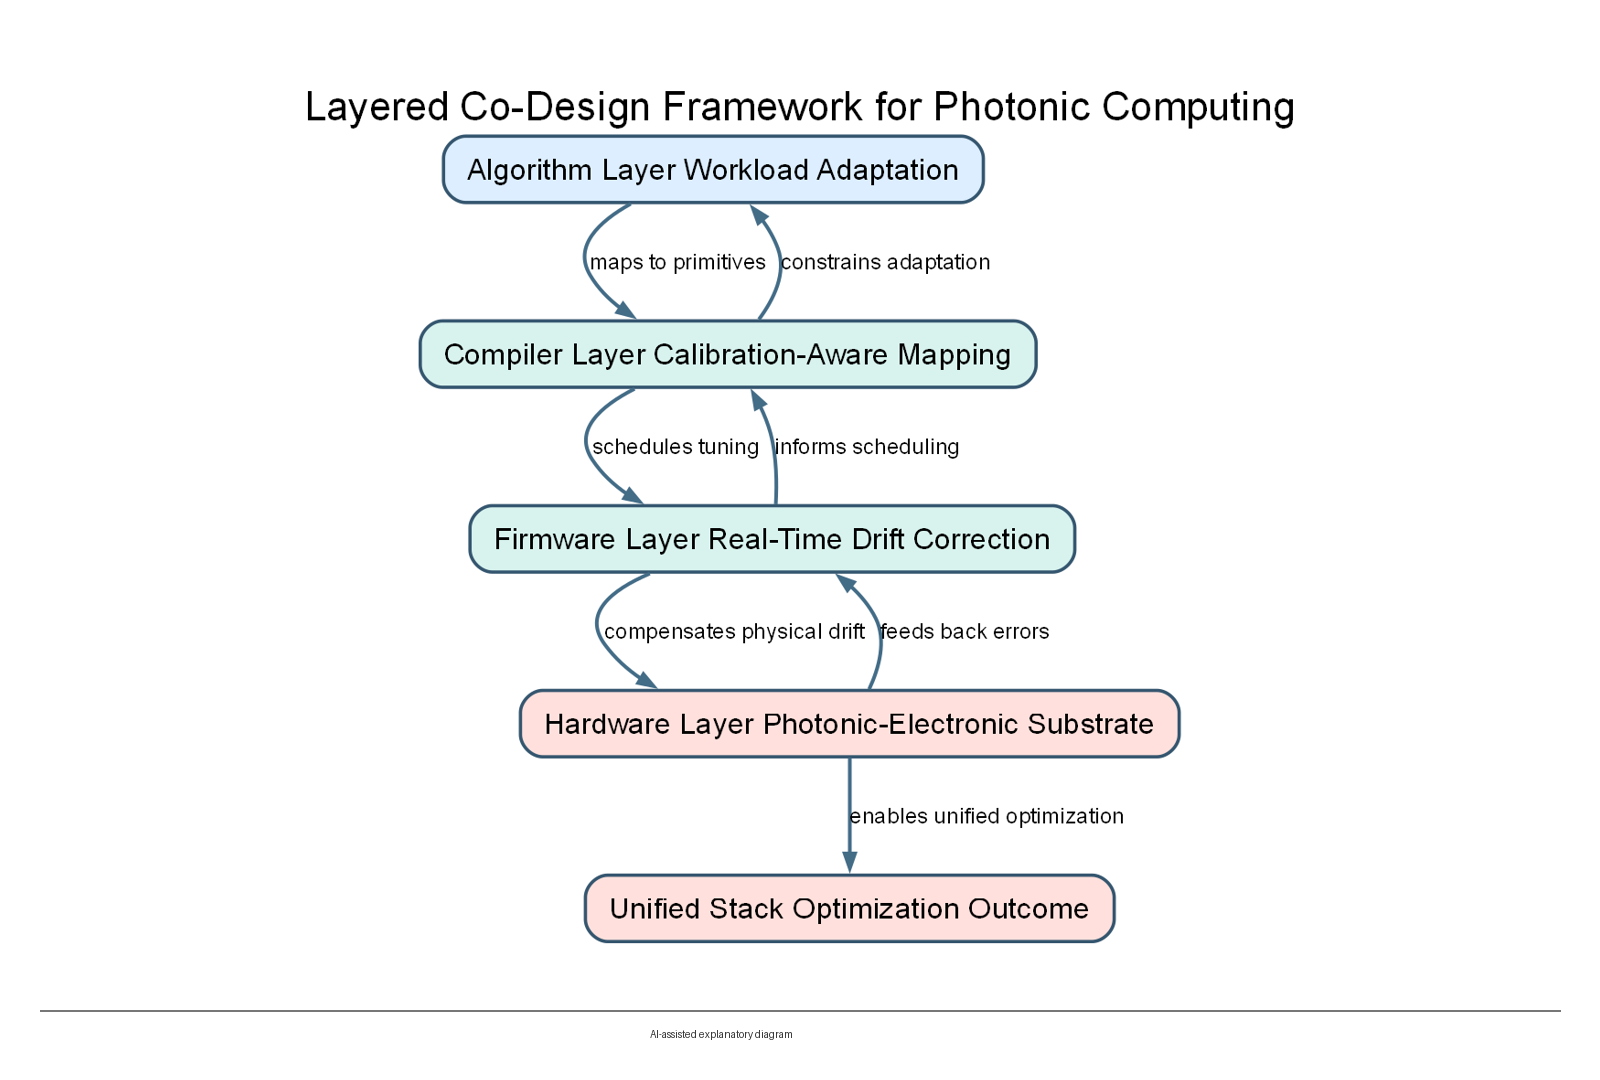
\includegraphics[width=0.9\linewidth,height=\textheight,keepaspectratio,alt={Layered Co-Design Framework for Photonic Computing. Co-design treats the entire stack as a unified optimization problem rather than optimizing components independently. AI-assisted explanatory diagram; not empirical evidence.}]{figures/02_FIG-GEN-004.png}
\caption{Layered Co-Design Framework for Photonic Computing. Co-design treats the entire stack as a unified optimization problem rather than optimizing components independently. AI-assisted explanatory diagram; not empirical evidence.}\label{fig:visual_02}
\end{figure}

特定的深度学习架构如今能够基于逆向设计这一基础概念,快速优化密集光互连网络所需的关键纳米光子元件。生成式深度神经网络和对抗自编码器作为强有力的工具,可将期望的光学响应直接映射为器件几何结构,从而规避了传统方法所耗时的迭代模拟过程。例如,条件生成对抗网络(CGAN)已被开发用于生成具有预设透射和反射特性的元原子的光刻掩模,进而促进了复杂超表面和光子晶体波导的构建。条件生成对抗网络(CGAN)已应用于超材料和光子晶体的逆向设计;具体而言,这些神经网络能够生成具有目标透射和反射特性的元原子光刻掩模,从而实现超表面和非线性光子晶体波导等复杂结构的制备。\citep{doi_10_1109_metamaterials62190_2024_10703328_b89eaef7} 同样,这些数据驱动方法正日益被用于设计集成硅纳米光子光栅,此类光栅对于 CMOS 兼容系统中的垂直光耦合至关重要。除精度之外,变分自编码器(VAE)和串联网络等先进方法也正因其能够产生多样化的设计候选方案并确保对工艺偏差的鲁棒性而受到评估,以满足实际中对具有平滑形貌和低深宽比结构的需求。此外,表征学习技术通过构建可复用且与物理机制无关的器件几何流形,缓解了计算瓶颈;这使得全局优化方案能够更高效地探索设计空间,而无须在每一步都承担全波电磁仿真的高昂成本。尽管这些架构显著加速了光谱调谐和相位控制元件的设计,但其对训练数据的依赖以及对工艺容差潜在的敏感性,凸显了进一步融入物理约束的必要性,这一问题将在下一节中予以探讨。\citep{doi_10_1109_metamaterials62190_2024_10703328_b89eaef7} \citep{doi_10_1109_cleo_europe_eqec52157_2021_9542763_c5b6331c} \citep{doi_10_29026_oes_2022_210012_27973a69} \citep{doi_10_1002_adom_202502062_d73a85e1}

深度学习架构加速了器件优化,然而纯数据驱动的神经网络往往难以泛化到其特定训练分布之外,限制了其在新型互连配置中的鲁棒性。为克服这一局限,混合算法应运而生,它将神经网络的全局搜索能力与传统优化方法的局部细化相结合。一种更为集成的解决方案是物理信息神经网络(PINNs),该方法将物理定律直接嵌入优化工作流,而非仅依赖数据模式。\citep{doi_10_1038_s41467_025_64624_3_42144da5} \citep{doi_10_3390_s25196242_b7203a7f} 通过将可微物理模拟器或基于伴随的方法纳入训练流程,这些模型实现了对复杂纳米光子结构的高效参数优化。例如,与标准方法相比,物理信息强化学习在设计自由形式超表面时展现出显著更高的样本效率;而其他框架则在未见过的设置中实现了更快的模拟速度和更低的预测误差。这种向物理约束设计的转变,确保了可扩展的光子计算织构在器件几何结构日益复杂的情况下仍能保持性能保真度。\citep{doi_10_1021_acsphotonics_2c00968_06a2e96b} \citep{s2_037e66f37189104d61c0d000de0cee202b7eec9e_d15b8018} \citep{doi_10_1515_nanoph_2023_0852_cb27a26f} \citep{doi_10_48550_arxiv_2209_10098_b3bedb78}

将物理信息设计转化为可大规模生产的组件,需要将逆向设计方法论适应于严格的晶圆厂制造约束。为此,通过将优化过程置于最小长度尺度和笔刷尺寸限制等硬性限制之下,强制实施可制造性,将设计任务转化为组合问题,并通过带有条件生成器的随机梯度优化进行近似求解。这确保了生成的光子组件在现有半导体工艺的大规模部署中保持可行性。此外,深度强化学习通过将器件调谐视为序列决策过程来实现自动化优化,使智能体能够学习满足高质量激光发射和电信所需严格谐振波长公差的策略。深度强化学习已应用于光子晶体的自动逆向设计和优化,特别是用于创建纳米级激光腔。\citep{doi_10_1515_nanoph_2022_0692_4b166807} 作为对这些感知约束方法的补充,深度学习模型作为前向预测的高效代理,学习结构参数与光学响应之间的映射关系,从而规避传统电磁仿真的计算开销。与必须为每个新设计目标重新启动的目标特定优化方法不同,这些代理模型跨问题泛化,能够在毫秒内预测最优结构,显著加速从仿真到制造的进程。这些进展共同弥合了理论性能与实际可制造性之间的差距,这是本章核心论点中可扩展光互连结构的前提条件。\citep{doi_10_1021_acsphotonics_2c00313_0d7d39c3} \citep{doi_10_1515_nanoph_2022_0692_4b166807} \citep{doi_10_29026_oes_2022_210012_27973a69} \citep{doi_10_1109_jphot_2022_3182050_3cfb78ba}

实现可扩展的光子织物最终取决于先进的材料平台,这些平台能够实现超越纯硅极限的密集、有源集成。异质后端(BEOL)集成通过将薄膜铌酸锂(TFLN)与有源硅光子学结合在单一衬底上解决了这一问题,该工艺克服了传统的芯片-晶圆键合挑战,从而将高性能收发器和计算加速器进行共封装。异质后端集成使得在单一衬底上将薄膜铌酸锂与有源硅光子学相结合成为可能,以实现单片光收发器。\citep{s2_9b444e84d20ae6e3d62d2d4df30268b5a53baad2_40af2cc9} 与无源硅电路不同,这种混合平台利用了TFLN固有的低损耗和卓越的调制效率,同时保留了成熟硅光子组件的CMOS兼容性。此类动态路由所需的有源控制源于铌酸锂独特的铁电特性,其中''电场极化''允许在室温下局部反转自发极化,从而在不使用过时的高温扩散工艺的情况下调控电光系数。\citep{s2_a1b7de5981aa9a6aa9f9bd0c4422d9b023fc454f_bec494c5} \citep{doi_10_1117_12_2654937_d0b4bc2b} 作为对这些体材料的补充,片上介电超表面提供了一种CMOS兼容机制来控制光场的自由度,充当紧凑、宽带操作(如卷积)中的任意波前整形器。尽管当前的调制器和探测器尚未达到其性能极限,但硅、TFLN和氮化硅的三层集成为复杂的系统级功能确立了清晰的路径,直接应对了限制全同态加密等新兴应用的内存带宽瓶颈。\citep{s2_9b444e84d20ae6e3d62d2d4df30268b5a53baad2_40af2cc9} \citep{doi_10_1126_science_abj4396_40f36a09} \citep{doi_10_1515_nanoph_2022_0294_1bd118d5} \citep{doi_10_1145_3806395_315ab915}

光互连现在正解决安全和人工智能计算领域中的关键瓶颈,这建立在先前描述的异质集成能力之上。在全同态加密(FHE)中,由于支持对加密数据直接进行计算以保护隐私敏感应用(如医疗保健),其性能往往因CKKS引导过程中的内存带宽限制而受到抑制。OptoLink架构通过在芯片级采用波分和空分复用,在128个光通道上提供高达1.6 TB/s的带宽,从而缓解了这一约束。该光学架构将延迟降低了300倍,并将引导吞吐量提高了多达11倍,有效地实现了大规模FHE加速的实际应用。人工智能领域的并行进展通过衍射光学神经网络(DONNs)得以实现,这些网络利用紧凑、无源的片上结构,为机器学习任务实现超高吞吐量和低功耗运行。互补的集成光子张量核进一步支持这些工作,通过在平铺光学架构中促进并行卷积处理和高带宽数据移动。总之,这些应用表明光互连提供了克服电气链路扩展性限制所需的带宽密度,但要充分发挥其潜力,需要解决接下来讨论的系统级热管理和协同设计挑战。\citep{doi_10_1145_3806395_315ab915} \citep{doi_10_1002_nap2_70098_8d5f2f8a} \citep{doi_10_1515_nanoph_2022_0423_38a2c3ec}

光互连有效解决了全同态加密等应用中的带宽瓶颈,然而其高密度集成引入了一个关键的物理限制:热串扰。在集成的热光衰减器和移相器中,芯片材料不可避免的热导率会导致热量从一个组件扩散到邻近组件,产生不必要的功率波动,从而限制了工作能力并可能导致信号路由错误。尽管已提出诸如三维沟槽或掺杂硅加热器等策略来局域化热效应,但现有设计往往存在占用面积大、功耗高或依赖与标准 CMOS 工艺不兼容的外部散热器等问题。这种器件级的不稳定性要求采用一种更广泛的协同优化方法,即将孤立进行的逆向设计与系统级架构约束紧密耦合。随着光子神经网络的规模扩大,众多光学模块中损耗、色散和噪声的累积需要硬件资源和软件工具共同管理这些热和损耗瓶颈。因此,要实现可扩展光子计算的全部潜力,必须对器件制造和系统架构进行协同设计,以缓解威胁高密度光网络可靠性的物理干扰。\citep{doi_10_1109_access_2020_3013116_8fec1fb2} \citep{doi_10_1145_3806395_315ab915} \citep{doi_10_3390_nano14080697_c372a140}

前述讨论强调了热串扰和架构协同设计是当前的直接障碍,然而关于光互连网络终极可扩展性的两个根本问题仍未解决。首先,尽管 OptoLink 等具体实现表明,光子芯粒架构可实现 1.6 TB/s 的带宽,并在全同态加密工作负载下将延迟降低至电子网络的 300 分之一,但现有资料尚未确证这些优势能否在更广泛的芯片间及板间扩展场景中,转化为能效(每比特能量)和带宽密度方面持续的数量级提升。其次,设计方法论中存在关键缺口:当前的机器学习方法似乎严重偏向于器件级优化,而非将互连网络与计算加速器直接集成所需的全面系统级协同设计。虽然 OptoLink 成功利用波分复用和空分复用技术,在特定平台上将启动吞吐量提高了高达 11 倍,但现有的逆向设计框架能否从优化孤立器件演进为管理分布式光子计算系统的复杂权衡,仍是一个悬而未决的问题。解决这些不确定性对于从有前景的点对点解决方案过渡到本章论点所展望的成熟可部署技术至关重要。\citep{doi_10_1145_3806395_315ab915}

\section{可扩展光子计算现状:综合、基准测试缺口与轨迹评估}\label{ux53efux6269ux5c55ux5149ux5b50ux8ba1ux7b97ux73b0ux72b6ux7efcux5408ux57faux51c6ux6d4bux8bd5ux7f3aux53e3ux4e0eux8f68ux8ff9ux8bc4ux4f30}

可扩展光子计算经历了一场根本性的范式转变,即从基于直觉的设计转向数据驱动的反向设计;这一方法论的演进对于突破传统方法所面临的几何复杂度极限至关重要。反向设计逆转了传统的仿真工作流程,利用优化算法和人工智能根据所需的光学响应直接确定器件几何结构,从而实现了人类启发式方法往往难以发现的非直观结构。\citep{doi_10_1117_12_3066105_d6297c38} \citep{doi_10_48550_arxiv_2506_18627_e2696034} 这一转变由深度学习架构驱动,其中判别模型学习物理参数与光学光谱之间的复杂映射关系,以规避重复且计算成本高昂的全波电磁仿真。例如,双向神经网络已展现出在数小时内完成训练收敛的能力,并随后可在毫秒级时间内生成有效的纳米光子布局(如开口环谐振器)。尽管生成模型通过学习到的潜在空间采样多样化的最优设计,进一步扩展了这种能力,但该方法仍面临局限:具体而言,初始训练阶段需要大量源自耗时仿真的标注数据集,且所得器件的性能被限制在其训练分布范围内。尽管存在这些计算开销,但这种人工智能驱动的基础对于产生系统集成所需的优化组件至关重要,也为下文将讨论的、旨在进一步扩展这些设计的快速仿真架构奠定了基础。\citep{doi_10_1515_nanoph_2021_0660_2d91a441} \citep{doi_10_1515_nanoph_2024_0536_4b6631ba}

神经算子作为一种关键架构应运而生,旨在加速光子仿真,其通过学习函数空间之间的映射而非固定的输入-输出对来实现这一目标,这建立在前述部分确立的数据驱动逆向设计基础之上。与传统回归高维向量的代理模型不同,DeepONets 等框架近似能够接受函数值输入(如边界条件或源项)的非线性算子,使其能够在几乎不增加成本的情况下评估新场景,同时保持可微性以支持基于梯度的优化。\citep{doi_10_48550_arxiv_2406_05072_c02ad5f4} \citep{doi_10_1122_8_0000908_e28c4124} 为了进一步解决传统时域有限差分求解器的计算延迟问题,最近的进展引入了尊重麦克斯韦方程内在时空因果约束的物理启发动态卷积架构。这些模型通过采用阶段专用子模型和跨阶段隐藏状态传播,减轻了自回归预测中典型的分布偏移和累积 rollout 误差,确保光场预测与真实动力学一致且不违反物理局域性。通过将静态矩阵乘法替换为捕捉介电常数依赖波传播的机制,这些可微仿真器显著降低了大规模设计任务相关的开销,直接解决了当前阻碍光子系统公平基准测试和可扩展部署的计算瓶颈。\citep{doi_10_48550_arxiv_2601_00199_c689b34d} \citep{doi_10_48550_arxiv_2406_17810_813bd2a3}

尽管神经算子和可微分模拟器加速了设计循环,但仍需将约束直接嵌入学习过程,以确保生成的几何结构在物理上有效且可制造。物理信息神经网络(PINNs)通过自动微分将控制物理方程直接纳入训练目标,从而提供硬约束;与纯粹数据驱动的黑盒模型相比,这提高了逆向设计光子器件的物理一致性和可靠性。\citep{doi_10_48550_arxiv_2606_12337_68b62bfa} \citep{doi_10_48550_arxiv_2603_09359_098af542} 这种人工智能与物理引导框架的融合,为电磁和纳米光子系统的设计与优化开辟了变革性途径,使稳健的工具能够应对光散射工程和超构光学中长期存在的挑战。为了弥合理论性能与实际部署之间的差距,这些方法日益受到严格的代工厂制造限制(如最小特征尺寸)的约束,从而将设计任务转化为可通过无约束随机梯度方法求解的组合优化问题。通过利用条件生成器产生可行设计,并采用直通估计器进行反向传播,逆向设计方法能够生成兼具高性能和可制造性的光子器件几何结构,直接解决了可扩展集成的关键障碍。然而,这些硬约束架构的有效性取决于能否解决多因果失效模式,包括频谱偏差和优化失衡;若不能解决这些问题,即使物理信息残差看似已最小化,仍可能导致损失权重崩溃。\citep{s2_cc39d5405a933620426d86298fa8fe4cd51915c5_27626ee3} \citep{s2_037e66f37189104d61c0d000de0cee202b7eec9e_d15b8018} \citep{doi_10_1021_acsphotonics_2c00313_0d7d39c3}

物理信息约束确保了可制造性,然而其底层的逆向设计方法面临着深刻的计算障碍,这些障碍源于高维、非凸的参数空间,往往违背人类直觉。自动化优化框架在此至关重要,但它们遭遇了独特的效率极限:全局随机方法受困于维数灾难,因为采样需求呈指数级增长;而基于梯度的方案则在振荡的目标地形中面临收敛至局部最优的风险。除了这些算法挑战外,基于深度学习的模型还引入了显著的开销,表现为对超参数调整的敏感性以及缺乏针对制造变异鲁棒性的系统评估。此外,当前的物理信息机器学习方法通过双层和随机优化需求加剧了这一负担,增加了训练复杂度,并目前限制了其在大规模系统中的即时可扩展性。纯生成式方法带来了另一项独特挑战,这类方法将逆向设计视为通过深度生成模型或微调语言模型学习的直接映射问题。尽管具有吸引力,此类模型仍面临持久的''约束严格性缺口''(Constraint Rigor Gap),其特征是难以严格执行科学领域中至关重要的硬性物理或化学约束。当前的生成式框架通常在其损失函数中通过软惩罚或正则化来处理这些约束,导致仅能部分满足约束,且据报道研究中的可行性率低至 60-80\%。这些计算瓶颈表明,虽然组件保真度是可以实现的,但通往可扩展部署的道路受阻于优化效率低下,而非基本的物理极限。\citep{doi_10_48550_arxiv_2602_18148_e9c0a72b} \citep{doi_10_29026_oes_2022_210012_27973a69} \citep{doi_10_55041_ijsrem43509_b9a7bd5e} \citep{doi_10_48550_arxiv_2511_00070_bf8eda11}

在解决了逆向设计的计算开销问题后,这些方法如今能够通过片上介电超表面和异质集成实现具体的硬件落地。片上介电超表面已成为可扩展光子计算的关键技术,因为它们提供了一种独特的方案来调控片上光场的自由度,同时保持与标准 CMOS 制造工艺的兼容性。这种兼容性使得低损耗、宽带硅光子超表面能够作为模拟光子加速器,执行卷积等基本运算。与此同时,异质后端线(BEOL)集成平台已成功将薄膜铌酸锂(TFLN)与有源硅光子器件相结合,克服了芯片到晶圆键合及多层集成中的关键挑战。与以往仅限于无源电路的努力不同,该实现在单颗芯片上集成了高速锗光电探测器与高性能 TFLN 调制器,并利用成熟的硅光子设计工具包以促进复杂的系统级功能。为确保这些物理结构得到最优实现,基于代理模型的逆向设计工作流将标签拟合、工艺感知参数化和电磁散射解耦为独立阶段。该方法首先在矩阵空间中直接优化光学模块,随后通过伴随问题将算子转移至工艺感知器件,从而缓解了单环路联合优化中固有的非凸性,并显著降低了每个 epoch 的计算成本。综上所述,超表面调控、异质材料集成以及解耦设计工作流的这些进展,弥合了抽象算法需求与可制造光子系统之间的差距,为在完整的光学神经网络架构中评估其性能奠定了基础。\citep{doi_10_1515_nanoph_2022_0294_1bd118d5} \citep{s2_9b444e84d20ae6e3d62d2d4df30268b5a53baad2_40af2cc9} \citep{s2_753a5d83a96e0194da93bcb6f20fa0bd356e37fa_c11e3796}

集成衍射光子计算单元现已展现出作为特定人工智能工作负载加速器的可行性,尤其是全光学图表示学习。与传统电子处理器难以应对大规模深度神经模型的串行需求不同,这些光子基底利用高并行性和光速信号处理,能够处理编码实体间关系的复杂图结构数据。衍射光学神经网络(DONNs)是这一变革中的关键架构,它利用无源低功耗运行和可扩展的神经元数量,为推理任务实现超高吞吐量。然而,尽管自由空间和片上实现为智能计算提供了不同的路径,但实际部署仍面临重大障碍,包括复杂的光学配置、严苛的对准要求以及缺乏高效的光学非线性激活机制。为解决这些集成挑战,混合方法应运而生,例如仅将训练和非线性功能置于电域而保留光学读出的电 - 光转换系统,从而避免了限制速度的转换过程。虽然这些简化的光电设计减少了对校准的需求,并能在不移动物理组件的情况下实现重构,但 DONN 研究仍受限于制造公差和标准化基准的缺失,这为进一步审视阻碍其与电子替代方案进行公平比较的评估差距奠定了基础。\citep{doi_10_1126_sciadv_abn7630_4399f2ff} \citep{doi_10_1002_nap2_70098_8d5f2f8a} \citep{doi_10_1364_oe_462370_1269b480}

OptoLink 等系统级演示展现了光子互连的变革潜力,实现了高达 1.6 TB/s 的带宽和相较于电子网络 300 倍的延迟降低;然而,这些孤立的成功凸显了评估方法的关键碎片化问题。目前,ODNN 研究是否缺乏能够同时考虑不同光子模式下能量效率和计算保真度的标准化基准测试协议,仍是一个未决问题;这种缺失阻碍了与电子替代方案的公平比较。标准化基准测试要求对运行参数进行一致定义,例如特定波长范围(如 900 至 1100 nm)和偏转角,以便在不同逆向设计策略之间进行直接的性能比较。若缺乏此类共识,所报告的指标将依赖于具体语境,从而难以区分根本性的架构优势与优化伪影。因此,尽管加密机器学习等特定应用展现出前景,但 ODNN 研究目前仍缺乏必要的标准化框架,以严谨地确立可扩展的光子计算是否在更广泛的工作负载下持续优于电子系统。\citep{doi_10_1145_3806395_315ab915} \citep{doi_10_1515_nanoph_2023_0852_cb27a26f} \citep{s2_9b444e84d20ae6e3d62d2d4df30268b5a53baad2_40af2cc9}

针对已识别的基准测试空白,可扩展光子计算的发展轨迹如今表明其采用路径出现了明显的分化。尽管通用光子人工智能加速器因标准化评估协议尚未确立而仍属小众领域,但光互连凭借成熟的 CMOS 兼容性及即刻解决特定带宽瓶颈的能力,有望在数据中心率先实现广泛部署。这种分化在 OptoLink 等架构中得到了体现:该架构利用波长与空间分割复用技术,在芯粒尺度上提供超高吞吐量,实现了高达 1.6 TB/s 的带宽,并与传统电子网络相比将延迟降低了 300 倍。此类系统级协同设计(即人工智能同时驱动器件优化与硬件实现)从根本上改变了光学深度神经网络(ODNN)的研究范式,使其从以组件为中心的努力转向软件定义的纳米光子基础设施,从而实现了硬件与终端用户约束的解耦。然而,尽管这些互连技术在缓解全同态加密等工作负载的内存传输延迟方面展现出明显优势,但在现实条件下缺乏统一的''每操作能耗''和延迟度量标准,是否会阻碍光子人工智能加速器相对于其电子对应物的更广泛扩展,目前仍是一个悬而未决的问题。\citep{doi_10_1145_3806395_315ab915} \citep{doi_10_1016_j_pquantelec_2023_100469_e4974ca6}

\section{结论}\label{ux7ed3ux8bba}

综合前文对器件物理、架构基元及系统级集成的分析,可扩展光子计算的发展得出了一个明确结论:光学深度神经网络(ODNN)研究已超越了对单一''银弹''材料或器件的寻求。相反,实现实际部署的路径在于异构材料平台的战略融合以及严格的电子 - 光子协同设计。关于光子系统能否扩展以满足下一代计算需求这一核心问题,答案是肯定的,但其在运行域方面存在关键限制。光子计算似乎并未准备好全面取代用于通用逻辑或高精度训练的电子处理器。相反,其可行性确立于一个专用范围内,该范围以高吞吐量、低精度推理和超大数据带宽传输为特征;在此范围内,光固有的并行性和能效相较于基于电荷的电子学具有显著优势。

这一结论建立在综述全文阐明的基本权衡之上。硅光子学具有 CMOS 兼容性但电光响应较弱,而薄膜铌酸锂提供卓越的调制效率却以集成密度为代价,这种二元对立使得混合集成策略成为必要。现有证据表明,目前没有任何单一材料平台能同时满足规模、速度和能效的所有要求。因此,异质后端集成成为一个关键使能技术,允许不同材料在单一衬底上结合,以利用各自的优势。然而,若不解决规模化时出现的系统性瓶颈,这种物理上的融合是不足的。本综述指出,热串扰、级联插入损耗以及制造引起的变异是加剧的信号保真度退化障碍。这些物理限制不仅仅是可以通过改进制造工艺克服的工程难题;它们代表了约束可实现电路深度和控制复杂度的基本边界条件。

此外,无源光子介质中原生非线性的缺失对算法适用性施加了结构限制。虽然光子矩阵乘法引擎擅长线性代数运算,但对激活函数和权重更新依赖混合电子机制,引入了可能侵蚀理论性能增益的延迟和能量开销。这一现实强化了以下发现:纯光子解决方案目前不适合需要频繁梯度计算的动态训练工作负载。相反,最有前景的应用在于静态或缓慢变化的推理任务以及光互连网络,其中光学硬件的刚性符合计算需求。OptoLink 等架构在缓解全同态加密内存带宽瓶颈方面的成功表明,光互连代表了该技术最可立即部署的应用,与电链路相比,其在带宽密度上提供了数量级的提升。

展望未来,可扩展光子计算的发展轨迹将更少依赖于组件的进一步微型化,而更多取决于整体协同设计方法的采用。传统的孤立优化器件的方法,对于应对晶圆级系统复杂且非凸的设计空间而言,正日益显得力不从心。结合物理信息的机器学习与逆向设计工具,为自动化地将抽象的算法目标映射到可制造的器件几何结构提供了一条路径,从而有效地将硬件约束作为优化循环的组成部分。然而,目前评估方法的碎片化阻碍了这一潜力的实现。缺乏针对能量每操作和计算保真度的标准化基准测试(涵盖多种光子模式),不仅阻碍了与电子替代方案的公平比较,也延缓了社区在最佳实践上的共识形成。

总之,可扩展光子计算正处于一个转折点。基础物理原理和架构原语已得到充分理解,其在特定领域产生变革性影响的潜力也已明确。然而,弥合实验室演示与稳健的系统级部署之间的差距,需要范式的转变。未来的进展可能不再由器件性能的孤立突破所驱动,而是由先进材料平台、智能设计算法与严格系统级验证的协同整合所推动。通过采纳这些协同设计策略,并解决基准测试与标准化方面的元挑战,光学深度神经网络(ODNN)研究有望从充满希望的点解决方案,过渡到后摩尔定律时代所设想的成熟、可部署的基础设施。
